\documentclass{scrartcl}[12pt, halfparskip]
\usepackage[utf8x]{inputenc}
\usepackage[T1]{fontenc}
\usepackage[english]{babel}
\usepackage{amsmath, amssymb, amstext}
\usepackage{wrapfig}
\usepackage{float}
\usepackage{graphicx}
\usepackage{color}
\usepackage{booktabs}
\usepackage{xfrac}
%\usepackage{amsthm}
\usepackage{ntheorem}

%\theoremstyle{break}
\newtheorem{Definition}{Definition}
\newtheorem{Theorem}{Theorem}
\newtheorem{Lemma}{Lemma}



\usepackage{pgfplots}
\usepackage{tikz}
\usetikzlibrary{fit} 
\usetikzlibrary{external}
%\tikzexternalize % activate!
%\usetikzlibrary{patterns}
\usetikzlibrary{patterns,decorations.pathreplacing}


    \tikzset{
    	hatch distance/.store in=\hatchdistance,
    	hatch distance=10pt,
    	hatch thickness/.store in=\hatchthickness,
    	hatch thickness=2pt
    }
    
    \makeatletter
    \pgfdeclarepatternformonly[\hatchdistance,\hatchthickness]{flexible hatch}
    {\pgfqpoint{0pt}{0pt}}
    {\pgfqpoint{\hatchdistance}{\hatchdistance}}
    {\pgfpoint{\hatchdistance-1pt}{\hatchdistance-1pt}}%
    {
    	\pgfsetcolor{\tikz@pattern@color}
    	\pgfsetlinewidth{\hatchthickness}
    	\pgfpathmoveto{\pgfqpoint{0pt}{0pt}}
    	\pgfpathlineto{\pgfqpoint{\hatchdistance}{\hatchdistance}}
    	\pgfusepath{stroke}
    }
    \makeatother



\newcommand\raalign[2]{%Umrahmen einer align-Gl.
	\tikz[overlay,every node/.style={inner sep=-2pt,outer sep=0pt}]%
	\node[anchor=base west](g){\phantom{$\displaystyle #1\null=\null#2$}}%
	node[draw=blue!50!black,fill=white!10,fit=(g),inner sep=5pt]{};%
	#1#2}


\usepackage{empheq}
\newcommand*\widefbox[1]{\fbox{\hspace{2em}#1\hspace{2em}}}


\usepackage{caption}
\usepackage{subcaption}

\bibliographystyle{unsrt}

\setlength{\parindent}{0pt}

\newcommand{\todo}[1]{\textcolor{red}{TODO: #1}}
\newcommand{\bem}[1]{\textcolor{blue}{Bem.: #1}}


\title{Master Thesis}


\author{Jan Lammel}
\date{\today{}, Heidelberg}



\begin{document}

\begin{titlepage}
	\begin{center}
	
	\textsc{\large Ruprecht-Karls-Universit\"{a}t Heidelberg} \\[0.5cm]
	\textsc{\large Master Thesis}\\[1cm]
	
	\newcommand{\HRule}{\rule{\linewidth}{0.5mm}}
	\HRule \\[0.4cm]
	\huge \bfseries Ueberschrift
	\HRule 
	
	\vspace{11cm}
	
	\Large \textit{Jan Lammel }\\
	\Large \textit{Heidelberg, \today }\\ \vspace{0.5cm}
	\Large \textit{Supervisor:}
	
	\Large \textit{Prof. Dr. Dr. h. c. mult. Hans Georg Bock}\\
	\Large \textit{Dr. Andreas Sommer}
	
	\end{center}
\end{titlepage}

\newpage

\tableofcontents 
\newpage

 \pagenumbering{Roman} 
 

 \addsec{Abstract}
 bla bla bla
 
 
 \newpage

\addsec{Zusammenfassung}
blubb !

\newpage
\pagenumbering{arabic}

\section{Introduction}
In this thesis we examine so called phase change materials (PCM). A popular application are heating pads (see Fig. \textcolor{red}{X}) which are liquid in a fully charged state. Folding induces a phase change to a solid state where energy is released and therefore the temperature increases. They can be easily recharged by applying a temperature above the melting point (e.g. with boiling water). 

In general PCMs work as an energy buffer. Another application are industry processes to store the process heat for later usage [\textcolor{red}{X}]. Furthermore they can be used to optimize photovoltaic cells because their efficiency is temperature dependent and has a maximum at a certain point. PCMs are able to stabilize the temperature where the efficiency is maximal \cite{pcm_solar_cells}. 
As a last example we deal with insulations of houses. During the day when it is hot, the PCM becomes liquid and absorb heat from outside, so they work as a cooling system. On the contrary at night when it is cold outside the PCM becomes solid, releases heat and work as a heater [\textcolor{red}{X}]. 


An important physical quantity is the specific heat capacity $c_p$ which tells us at which temperature the phase transition occurs and how much energy can be stored. The major goal of this thesis is to simulate the measuring process of a differential scanning calorimetry (DSC) where a PCM undergoes a phase transition and perform a parameter estimation in order to get the PCM's specific heat capacity. \\
As we will see in more detail in section \ref{sec:physics_DSC} the common way of computing $c_p(T)$ from DSC measurement data yields different results depending on the heat rate, a measurement parameter. Since $c_p(T)$ is a material property this is unphysical and this issue is known as the smearing problem. \\
By applying the parameter estimation we aim to avoid this problem. Furthermore the heat rate is proportional to the time duration of the experiment. If we get the same $c_p(T)$ for all heat rates we are able to accelerate the measuring process and therefore the research on this materials drastically. 
 


\section{Physical Background}
\subsection{Physical quantities and phase transition}

First of all some important physical quantities will be introduced because they are crucial for further comprehension. A summary is shown in Table \ref{tab:important_physical_quantities} with the consistently used symbol in this thesis and the physical unit. \\
Heat $Q$ is the energy that flows from a warmer to a colder object because of the temperature difference. The heat flux density $\phi$ tells us how much heat flows through an unit area in one second. It can be computed by Fourier's law: $\phi = - \lambda \nabla T$. By considering a particular area this changes to the heat flux $\varPhi$. Heat conductivity $\lambda$ is a material property how much energy is transported on a distance of $1m$, unit area and temperature difference of $1K$ in one second.

\begin{table}[H]
	\centering
\begin{tabular}{| c | c | c |} \hline
	Quantity & Symbol & Unit \\ \hline
	Heat & $Q$ & $J$ \\[0.7ex]
	Heat flux density & $\phi$ & $\frac{W}{m^2}$ \\[0.7ex]
	Heat flux & $\varPhi$ & $W$ \\[0.7ex]
	Heat conductivity & $\lambda$ & $\frac{W}{m \cdot K}$ \\[0.7ex]
	Specific heat capacity & $c_p$ & $\frac{J}{kg \cdot K}$ \\[0.7ex]
	Enthalpy & $H$ & $J$ \\ \hline
\end{tabular}
\caption{Important physical quantities}
\label{tab:important_physical_quantities}
\end{table}



Probably the most important physical quantity for us is the specific heat capacity $c_p$ which is a temperature dependent material property that tells us how much energy is needed to increase the temperature of $1kg$ of this material by $1K$. Since we are primarily interested in the phase change we handle with the so called apparent specific heat capacity which includes a peak at the melting point with a certain area equal to the melting enthalpy. For a pure substance this peak would be ideally a Dirac delta function. A constant heat flux entering such a pure substance increases the temperature until phase change. Afterwards the heat is absorbed in order to perform the phase transition while the temperature stays constant. Finally after the phase change has finished the temperature increases again. In mixed substances like PE in our case with different lengths of the individual polymer chains or due to lattice defects the peak extends over a temperature range.

\todo{Hier Bild von diesem Prozess einfuegen???} 

\todo{Enthalpy $H$}


\subsection{Heat equation}
\label{sec:heat_equation}
\todo{Herleitung als Quelle Buch "Waerme- und Stoffuebertragung" \cite{lit:waerme_und_stoffuebertragung} und quasi abschreiben.} \\
Since we are dealing with heat transport in the measuring process the central equation in this thesis is the heat equation. \\
For the derivation we start with the continuity equation with sources and sinks

\begin{equation}
	\frac{\partial \rho_h}{\partial t} + \nabla \cdot J_q = 0
\end{equation}

where $\rho_h$ is the enthalpy density and $J_q$ is the heat flux density. We assume a constant pressure so it holds $dH = dQ$ such that a heat flux will only change the enthalpy.

\begin{equation}
	J_q = - \lambda \cdot \nabla T
	\label{eq:fouriers_law}
\end{equation}

The enthalpy density $\rho_h = \rho h$ expressed with the mass density $\rho$ and specific enthalpy $h$ and Fourier's law inserted in the continuity equation gives us

\begin{align}
	\frac{\partial (\rho h)}{\partial t} = \nabla \cdot \left[\lambda \cdot \nabla T\right] \\
	\Leftrightarrow \frac{\partial \rho}{\partial T} \frac{\partial T}{\partial t} h + \rho \frac{\partial h}{\partial T} \frac{\partial T}{\partial t} = \nabla \cdot \left[\lambda \cdot \nabla T\right] \\
	\Leftrightarrow \left( \frac{\partial \rho}{\partial T} h + \rho \frac{\partial h}{\partial T} \right) \frac{\partial T}{\partial t} = \nabla \cdot \left[\lambda \cdot \nabla T\right]
\end{align}

Using the definition of the specific heat capacity $c_p := \frac{dh}{dT}$ we get the final heat equation

\begin{equation}
	\left( \frac{\partial \rho}{\partial T} h + \rho c_p \right) \frac{\partial T}{\partial t} = \nabla \cdot \left[\lambda \cdot \nabla T\right]
\end{equation}

\todo{Pruefen lassen ob das physikalisch alles so stimmt...}



\subsection{Differential Scanning Calorimetry}
\label{sec:physics_DSC}
The measuring method of a heat flux into a sample over a certain temperature range is called Differential Scanning Calorimetry (DSC). 

\begin{figure}[H]
	\centering
	\begin{subfigure}{0.49\textwidth}
		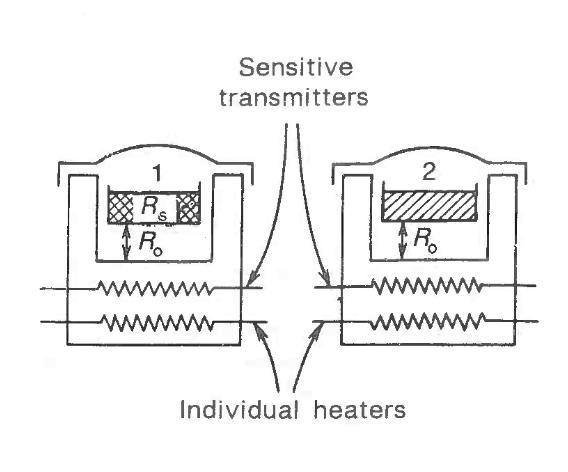
\includegraphics[width=1.\textwidth]{/home/argo/masterarbeit/thesis/images/dsc_principle.png}
		\caption{}
		\label{fig:DSC_power_compensated_principle}
	\end{subfigure}
	\begin{subfigure}{0.49\textwidth}
		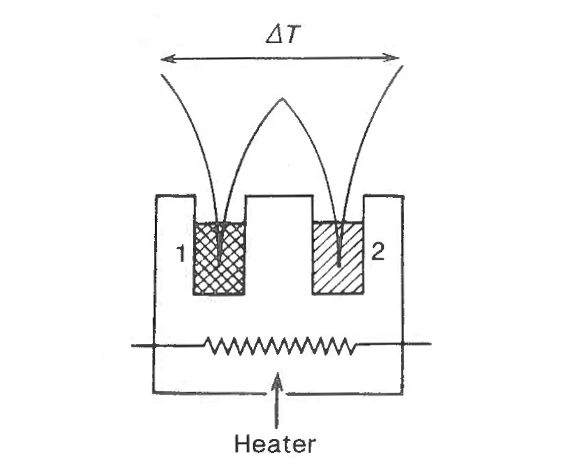
\includegraphics[width=1.\textwidth]{/home/argo/masterarbeit/thesis/images/dta_principle.png}
		\caption{}
		\label{fig:DTA_principle}
	\end{subfigure}
	\caption{}
\end{figure}


\subsubsection{power compensated DSC}
In the case of a power compensated DSC (Fig. \ref{fig:DSC_power_compensated_principle}) there are 2 seperated chambers for a reference and the sample. Both have individual heaters and temperature sensors such that a feedback control system keep the temperature in both chambers on the same value. Since we know the electrical power for heating we can deduce on the heat flux due to energy conservation. \\
\todo{Fuer was genau brauchen wir die Referenz?}




\subsubsection{heat flux DSC}
The heat flux DSC is based on differential thermal analysis (DTA, see Fig. \ref{fig:DTA_principle}). 
In DTA there is just one chamber in which both reference and sample are heated equally. 
Due to differences in the heat capacity of reference and sample a temperature difference dependent on their temperature will appear.
This can be used to find typical temperatures of known substances to identify the sample's components. \\
Unfortunately calorimetric properties like melting enthalpy are not accessible just from the temperature difference measurement. 
Note that the physical quantity measured is an electrical potential difference $\Delta U$ which is assumed to be proportional to the temperature difference due to the Seebeck effect. \\

\begin{figure}[H]
	\centering
	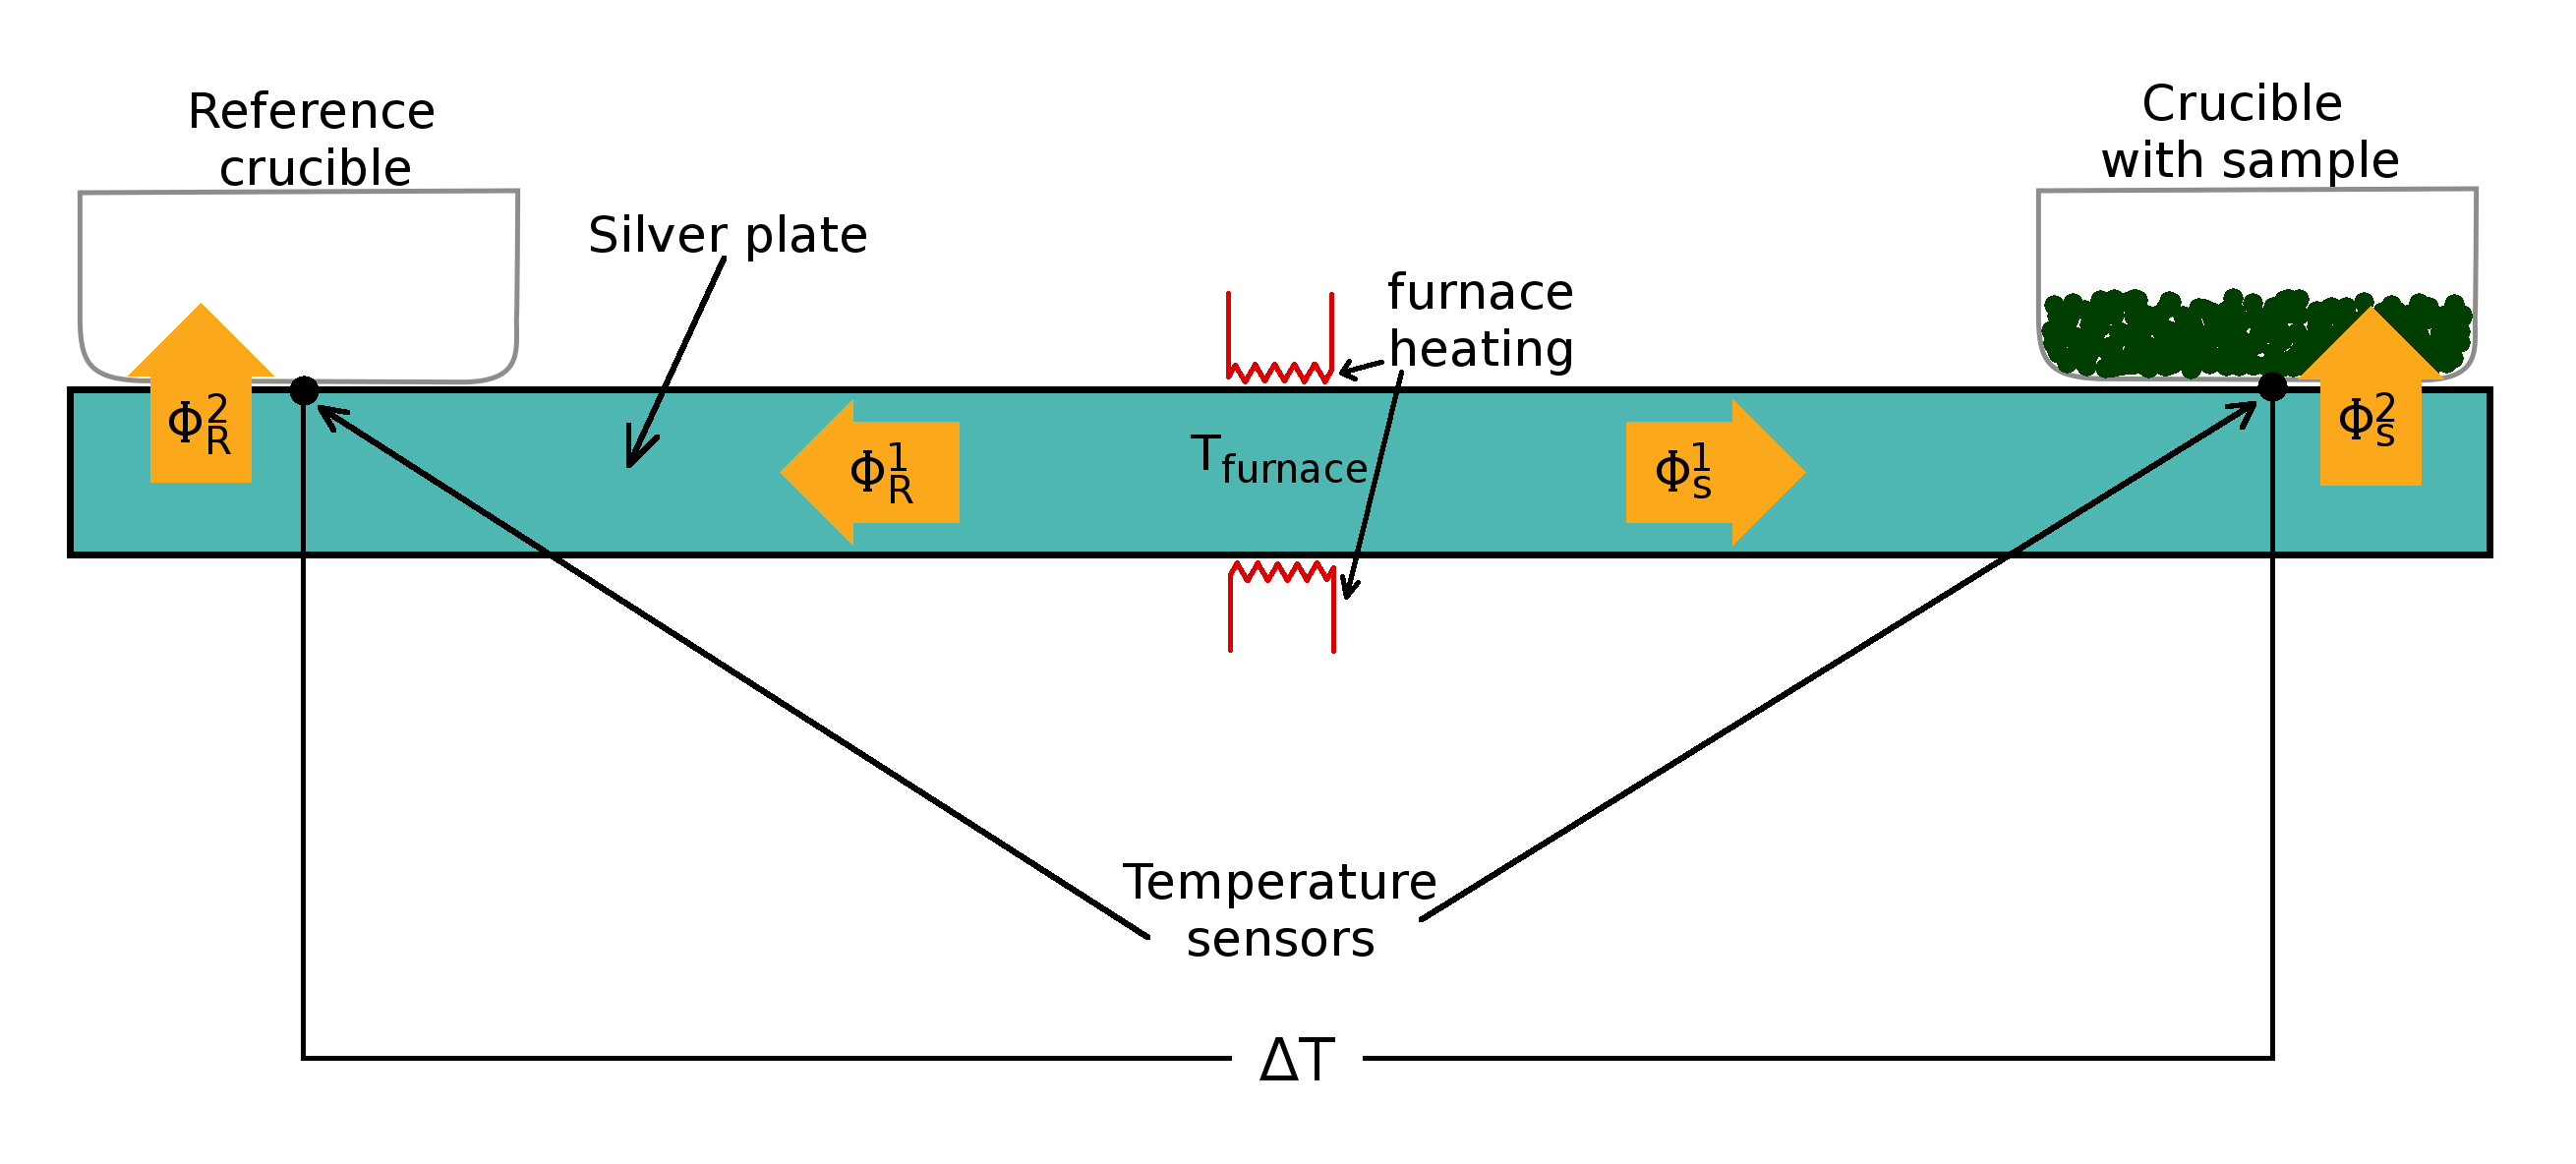
\includegraphics[width=1.\textwidth]{/home/argo/masterarbeit/thesis/images/dsc_funktionsprinzip.png}
	\caption{Principle experimental scheme of DSC which has been used for measurements.}
	\label{fig:heat_flux_DSC}
\end{figure}

The heat flux DSC (see Fig. \ref{fig:heat_flux_DSC}) extends now DTA by computing the heat flux into the sample $\Phi$ from the temperature difference using an additional calibration. 
Pure materials with known melting temperature $T_{\text{Kal}}$ and melting heat $\Delta Q_{\text{Kal}}$ are measured, giving the measuring signal $\Delta U(t)$ with a peak at the phase change. 
The area of this peak is assumed to be proportional with constant $sens$ called sensitivity to the melting heat due to

\begin{equation}
	A_{\Delta U} \propto \Delta Q_{\text{Kal}} \quad \Rightarrow \quad sens = \frac{A_{\Delta U}}{\Delta Q_{\text{Kal}}}
\end{equation} 

This is done for a set of calibration materials such that we get a mapping $sens(T)$ by interpolating the data points $(T_{\text{Kal,i}}, sens_i)$, see Fig. \ref{fig:dsc-calibration_sens(T)}.

\begin{figure}[H]
	\centering
	\begin{subfigure}{0.45\textwidth}
		\centering
		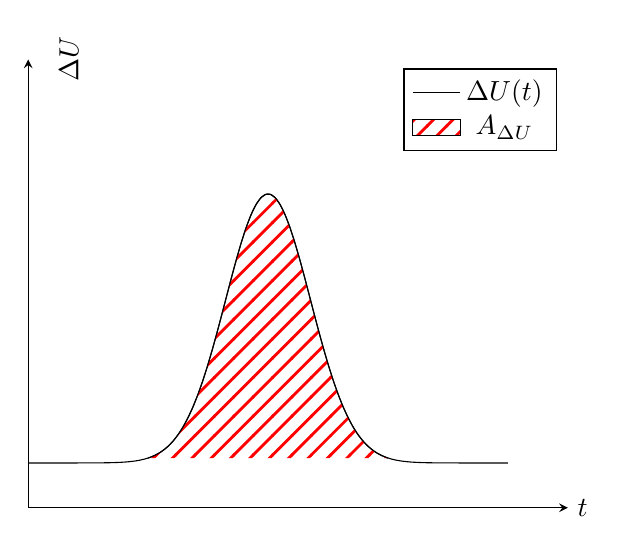
\begin{tikzpicture}
		\begin{axis}[domain=-1:7,
		samples=100,
		ymin=0, ymax=5	,	
		xmin=-1, xmax=8,	 
		axis lines=left,
		xtick=\empty,
		ytick=\empty,
		xlabel=$t$, xlabel style={at=(current axis.right of origin), anchor=west},
		ylabel=$\Delta U$, ylabel style={at=(current axis.above origin), anchor=south}]
		
		\addplot+[color=black,
		mark=none] {3*exp(-(x-3)^2) + 0.5};
		\addlegendentry{$\Delta U(t)$}
		\addplot+[mark=none,
		domain=1:5,
		samples=100,
		pattern=flexible hatch,
		hatch distance=8pt,
		hatch thickness=1pt,
		draw=black,
		pattern color=red,
		area legend]
		{3*exp(-(x-3)^2) + 0.5};
		\addlegendentry{$A_{\Delta U}$}
		\end{axis}
		\end{tikzpicture}
		\caption{}
		\label{fig:dsc-calibration_dU(t)}
	\end{subfigure}
	\hfill
	\begin{subfigure}{0.45\textwidth}
		\begin{tikzpicture}
		\begin{axis}[domain=-1:6.3,
		samples=100,
		ymin=0, ymax=5	,	
		xmin=-1, xmax=8,	 
		axis lines=left,
		xtick={2, 4},
		xticklabels={$T_{Kal,i}$, $T_{Kal,i+1}$},
		ytick=\empty,
		xlabel=$T$, xlabel style={at=(current axis.right of origin), anchor=west},
		ylabel=$sens$, ylabel style={at=(current axis.above origin), anchor=south}
		]
		
		\addplot+[color=black, mark=none] {3 - 0.1*x - 0.005*x^2};
		\addplot[only marks, mark=x, color=black] 
		table {0 3.
			1 2.9
			2 2.8
			4 2.55
			5 2.4
		};
		\end{axis}
		\end{tikzpicture}
		\caption{}
		\label{fig:dsc-calibration_sens(T)}
	\end{subfigure}
	\caption{\todo{!!!}}
\end{figure}

With the mapping $\Phi(T_{ref}) = \frac{\Delta U(T_{ref})}{sens(T_{ref})}$ the heat flux into the sample then can be computed for a measurement signal $\Delta U$. 




\subsubsection{Smearing Problem}
The common way to perform the DSC calibration, measurement and compute the specific heat capacity $c_p$ is described in detail in DIN 11357 \cite{DIN_11357}. By assuming a proportionality between the heat flux into the sample and the sample's heat capacity one gets the equation

\begin{equation}
	c_p^S(T) = c_p^{R}(T) \cdot \frac{m^R}{m^S} \cdot \frac{\Phi^S(T) - \Phi^0(T)}{\Phi^R(T) - \Phi^0(T)}
	\label{eq:c_p_formula_DIN}
\end{equation}

where $S$ and $R$ denote the sample respectively reference. Reference means here a material with known specific heat capacity $c_p^R(T)$, not to be mistaken with the reference side of the experimental setup. In our case this reference material is Saphir. $m$ is the mass and $\Phi^0$ is the heat flux if both crucibles are empty to compensate asymmetries. \\
In Fig. \ref{fig:heat_flux_measurements} the measurement data of the heat flux into the PCM is shown for all heat rates dependent on the temperature at the reference crucible. Using \eqref{eq:c_p_formula_DIN} the computed specific heat capacities for the PCM are shown in Fig. \ref{fig:c_p_DIN_formula}. As one can see for higher heat rates the peak position shifts to higher temperatures and furthermore the peak is smeared out. This is known as the smearing problem since $c_p$ is a material property and must be equal for all heat rates.


\begin{figure}[H]
	\begin{subfigure}{0.49\textwidth}
		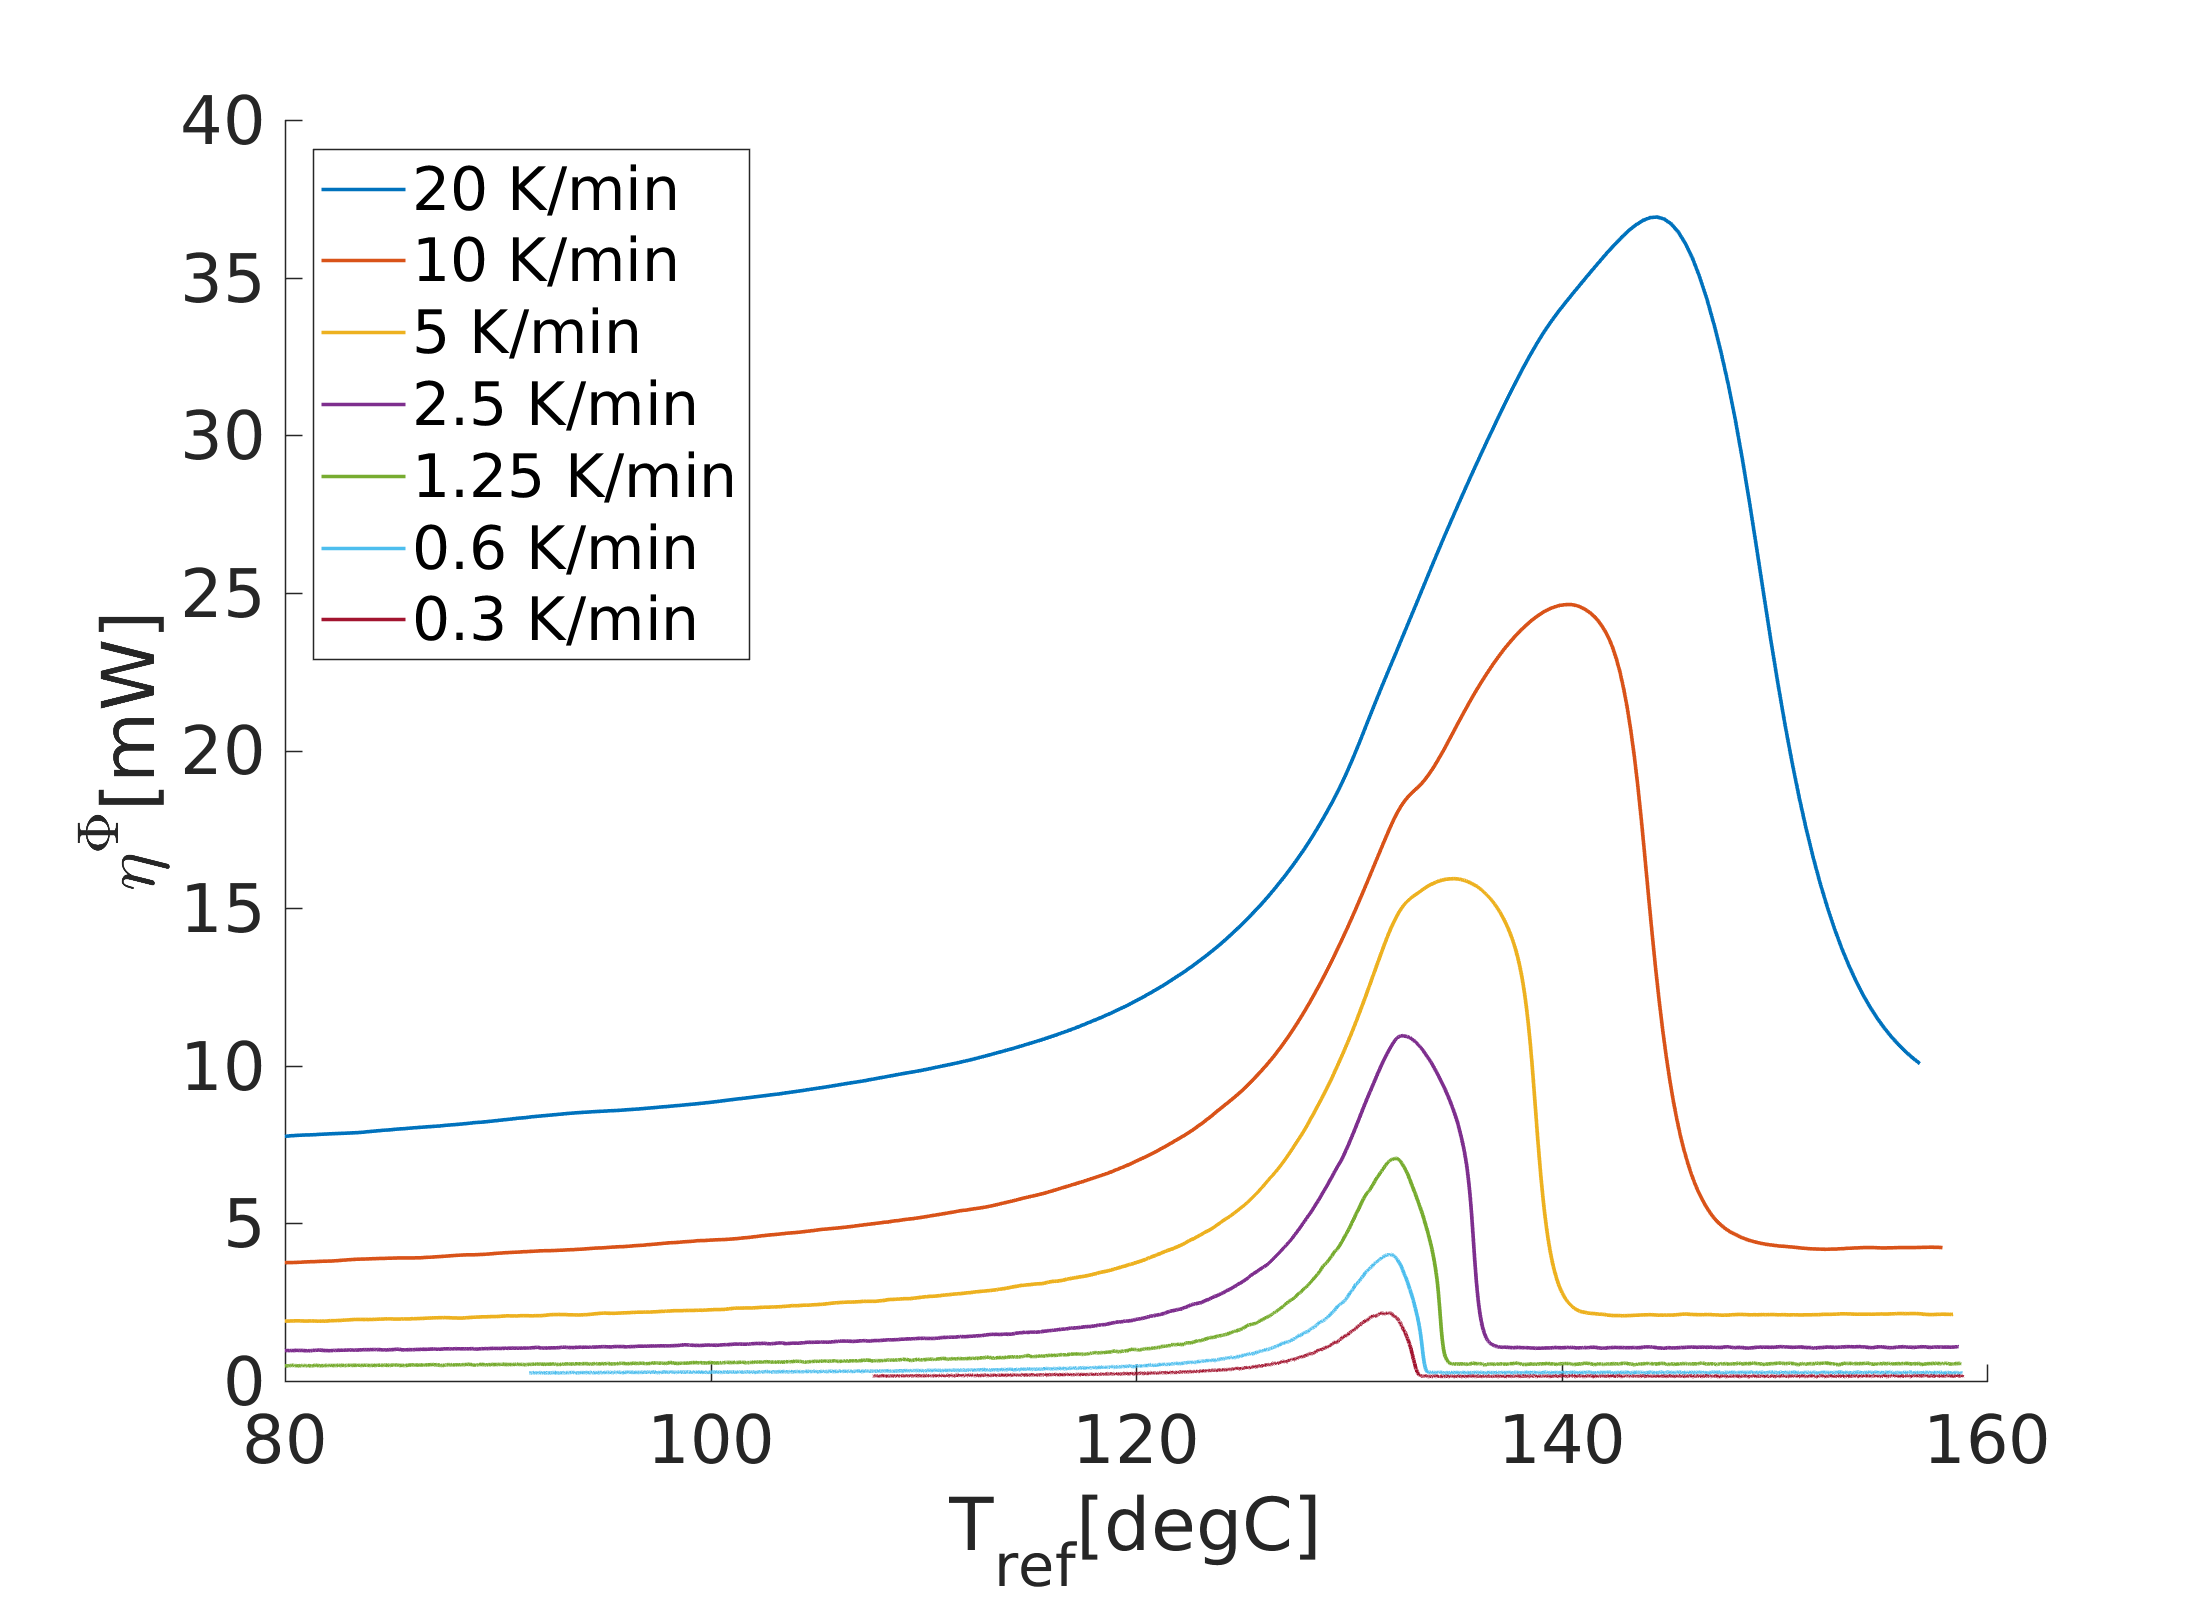
\includegraphics[width=1.\textwidth]{/home/argo/masterarbeit/vortrag/images/heat_flux_measurement.png}
		\caption{}
		\label{fig:heat_flux_measurements}
	\end{subfigure}
	\begin{subfigure}{0.49\textwidth}
		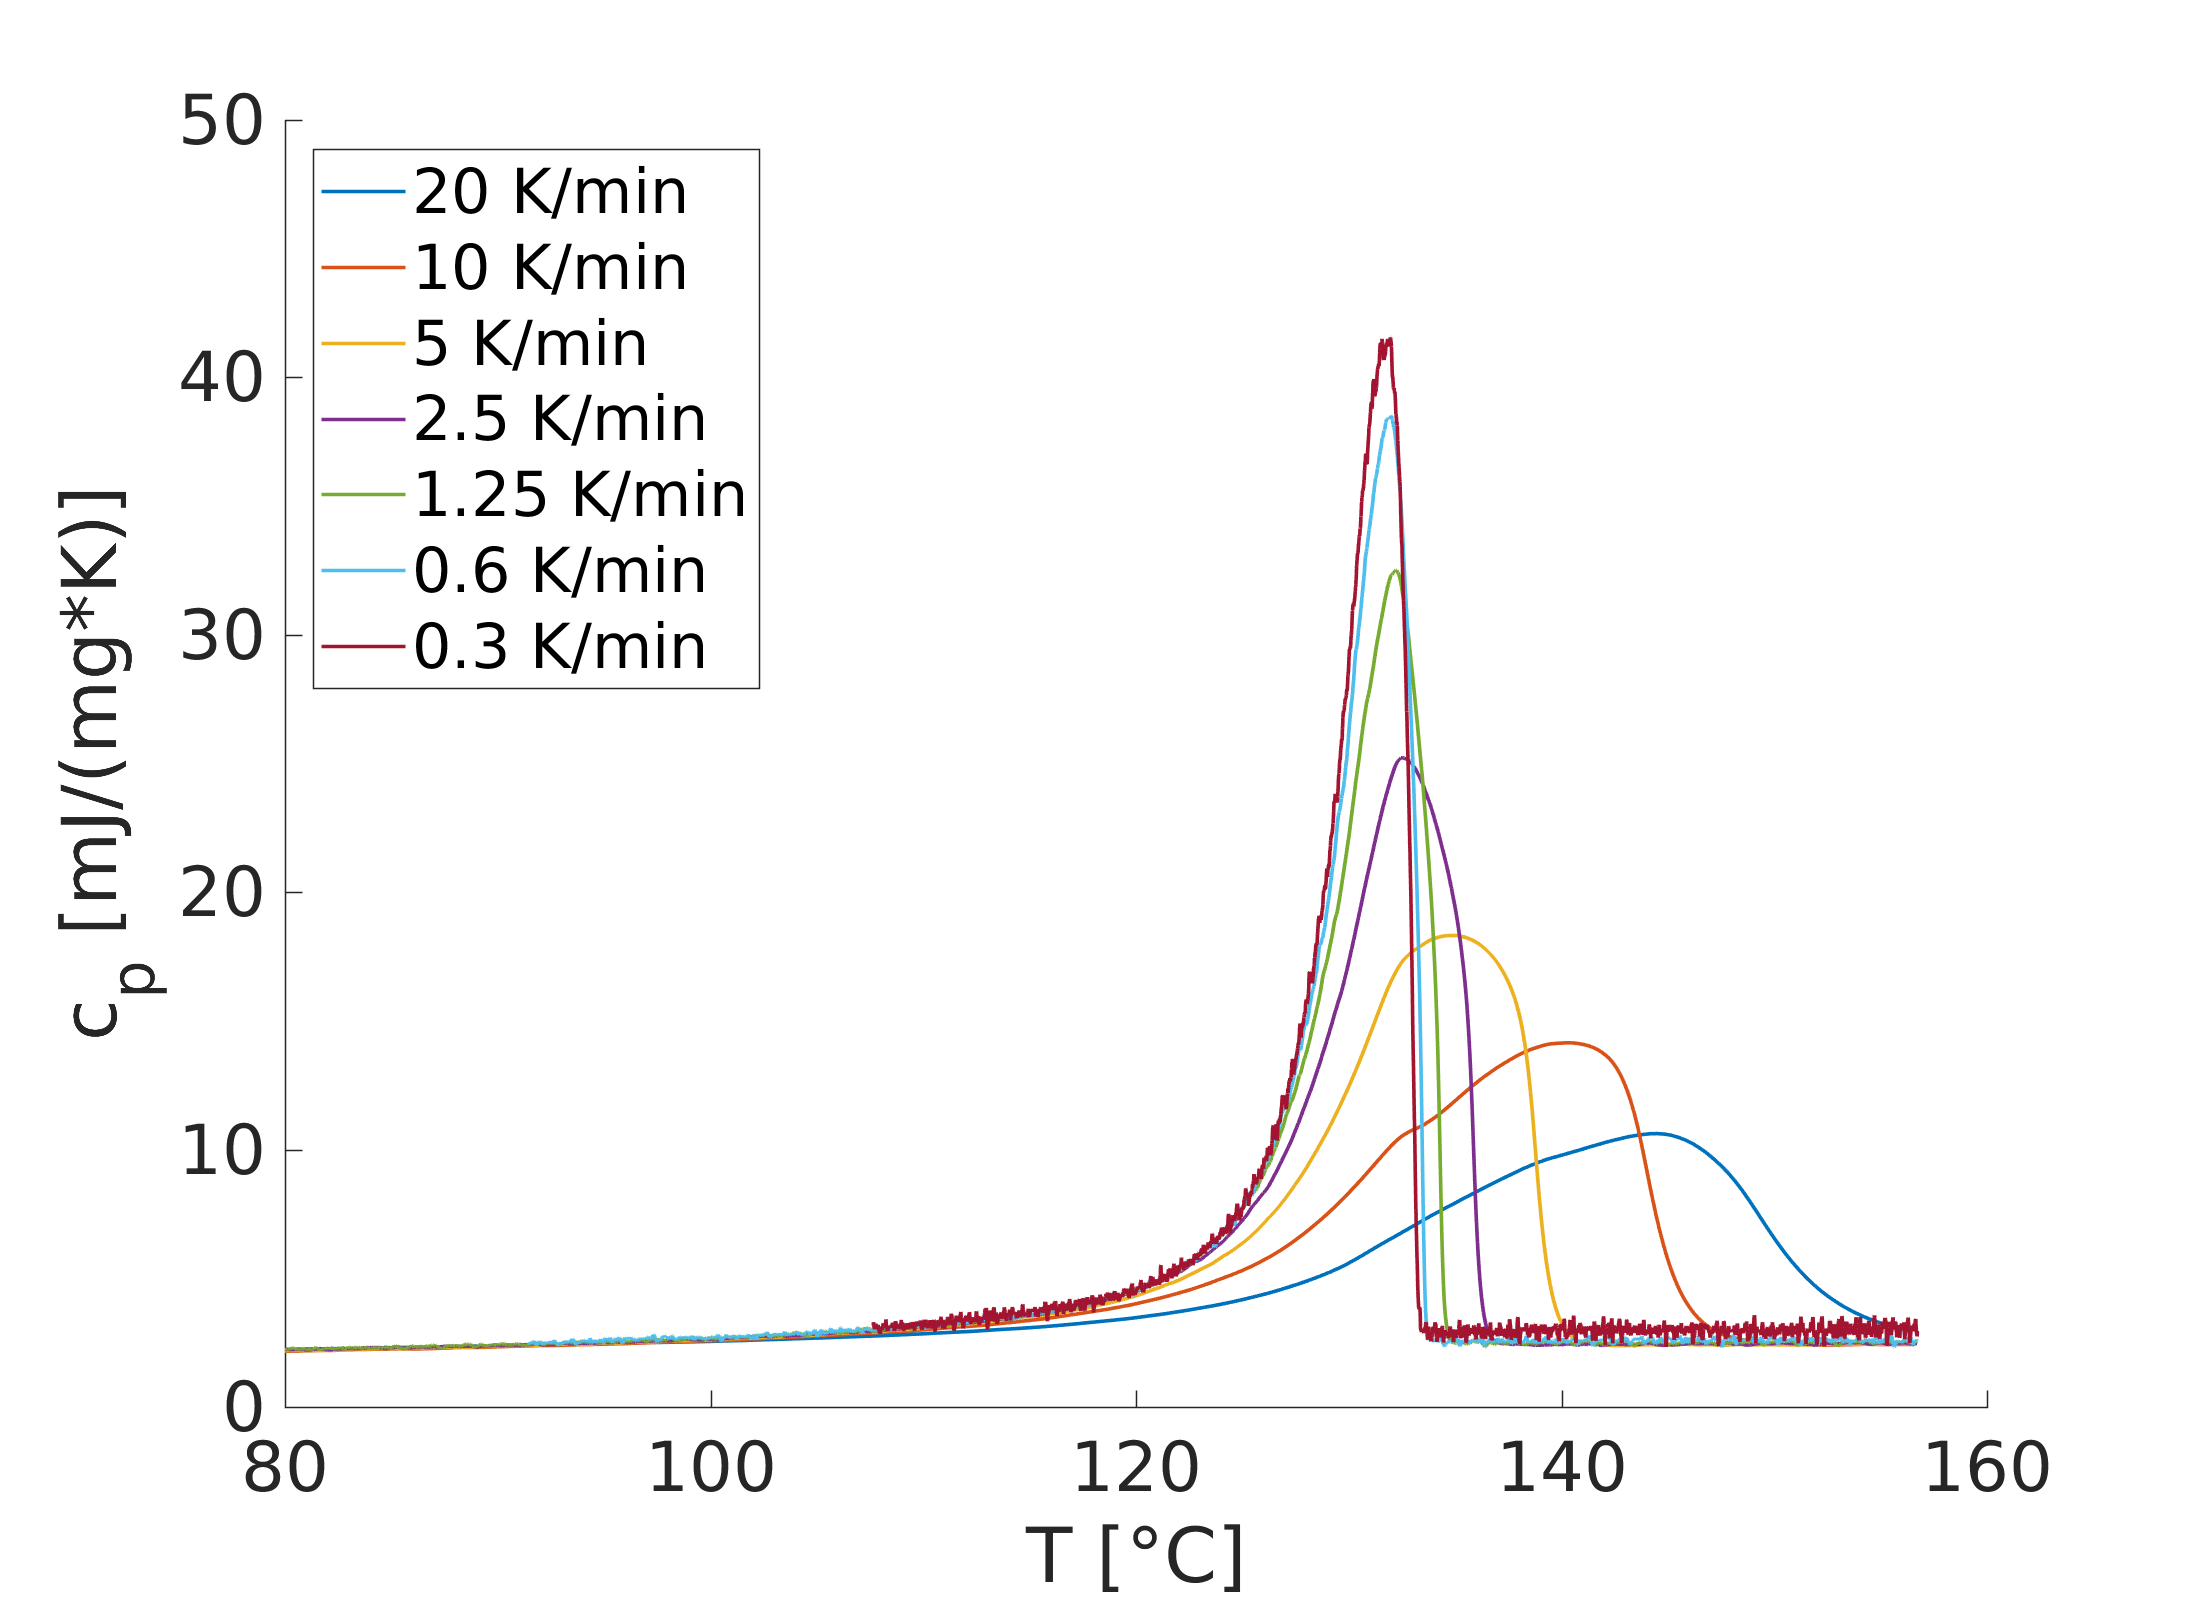
\includegraphics[width=1.\textwidth]{/home/argo/masterarbeit/vortrag/images/c_p_DIN_formula.png}
		\caption{}
		\label{fig:c_p_DIN_formula}
	\end{subfigure}
	\caption{\todo{Reihenfolge Heizraten richtig}}
\end{figure}


\newpage
\section{Mathematical Background}

\subsection{Derivative generation}
In the context of continuous optimization we are dependent on derivative information in order to minimize some function. 
There are several possibilities to obtain these derivatives. We will introduce here the concept of finite differences and automatic differentiation which were used in this thesis. 
Beside them the methods of symbolic- and complex step-differentiation exist and are explained in detail in \cite{diss_jan}.

\subsubsection{Finite Differences}
\label{subsubsec:finite_differences}
Derivatives generated by finite differences are needed beside the optimization task also in the spatial discretization of a partial differential equation which will be explained in more detail in section \ref{subsection:pde_discretization}.
They can be derived easily from Taylor-series expansion. Considering the function $f: \mathcal{R} \rightarrow \mathcal{R}^m$ the Taylor series looks as follows:


\begin{equation}
f(x+h) = f(x) + h \cdot \frac{\partial f}{\partial x}(x) + \mathcal{O}(h^2)
\end{equation}

Reordering gives the one-sided derivative approximation

\begin{equation}
\frac{\partial f}{\partial x}(x) = \frac{f(x+h) - f(x)}{h} + \mathcal{O}(h^2)
\end{equation}

Regarding the Taylor series up to order two in both directions of the domain of definition,

\begin{subequations}
	\label{eq:finite_differences_taylor_exp}
	\begin{align}
	f(x+h) = f(x) + h \cdot \frac{\partial f}{\partial x}(x) + \frac{h^2}{2} \cdot \frac{\partial^2 f}{\partial^2 x}(x) + \mathcal{O}(h^3) \label{eq:finite_differences_taylor_exp_+} \\
	f(x-h) = f(x) - h \cdot \frac{\partial f}{\partial x}(x) + \frac{h^2}{2} \cdot \frac{\partial^2 f}{\partial^2 x}(x) + \mathcal{O}(h^3)  \label{eq:finite_differences_taylor_exp_-}	
	\end{align}
\end{subequations}


subtract both equations and reorder again we get

\begin{equation}
\frac{\partial f}{\partial x}(x) = \frac{f(x+h) - f(x-h)}{2 h} + \mathcal{O}(h^3)
\end{equation}

which has a higher error order but at the expense of two function evaluations. \\

Second order derivatives can be gained analogously by adding \eqref{eq:finite_differences_taylor_exp_+} and \eqref{eq:finite_differences_taylor_exp_-}:

\begin{equation}
\frac{\partial^2 f}{\partial^2 x}(x) = \frac{f(x-h) - 2 \cdot f(x) + f(x+h)}{h^2} + \mathcal{O}(h^3)
\label{eq:finite_difference_2nd_der}
\end{equation}





In the spatial discretization of partial differential equations one often choose a finer grid for areas of interest. So for the resulting non-equidistant grid (see Fig. \ref{fig:2_point_formula_illustration}) one needs a more general formula which is derived by considering again the Taylor expansion





\begin{subequations}
	\label{eq:finite_differences_taylor_exp_non-homogenous}
	\begin{align}
	f(x-h) = & f(x) - h \cdot \frac{\partial f}{\partial x}(x) + \frac{h^2}{2} \cdot \frac{\partial^2 f}{\partial^2 x}(x) + \mathcal{O}(h^3) \label{eq:finite_differences_taylor_exp_non-homogenous_1} \\
	f(x+\alpha h) = & f(x) + \alpha h \cdot \frac{\partial f}{\partial x}(x) + \frac{\alpha^2 h^2}{2} \cdot \frac{\partial^2 f}{\partial^2 x}(x) + \mathcal{O}(h^3)  \label{eq:finite_differences_taylor_exp_non-homogenous_2}
	\end{align}
\end{subequations}



Multiplying \eqref{eq:finite_differences_taylor_exp_non-homogenous_1} with $\alpha$ and adding \eqref{eq:finite_differences_taylor_exp_non-homogenous_2} gives

\begin{align}
\alpha f(x-h) + f(x+\alpha h) = \alpha f(x) + \alpha \frac{h^2}{2} \frac{\partial^2 f}{\partial^2 x}(x) + f(x) + \frac{\alpha^2 h^2}{2} \frac{\partial^2 f}{\partial^2 x}(x) + \mathcal{O}(h^3)  \\
\Leftrightarrow (\alpha+1) \frac{\alpha h^2}{2} \frac{\partial^2 f}{\partial^2 x}(x) = \alpha f(x-h) - (\alpha+1) f(x) + f(x+\alpha h) + \mathcal{O}(h^3) 
\end{align}

\begin{equation}
\Leftrightarrow \frac{\partial^2 f}{\partial^2 x}(x) = \frac{1}{h^2} \left[ \frac{2}{1+\alpha} f(x-h) - \frac{2}{\alpha} f(x) + \frac{2}{\alpha (\alpha+1)} f(x+\alpha h) \right] + \mathcal{O}(h^3) 
\label{eq:2_point_formula_inhomogeneous}
\end{equation} \\

Note that for a homogeneous grid ($\alpha=1$) this is obviously equal to \eqref{eq:finite_difference_2nd_der}. \\

\begin{figure}[H]
	\centering
	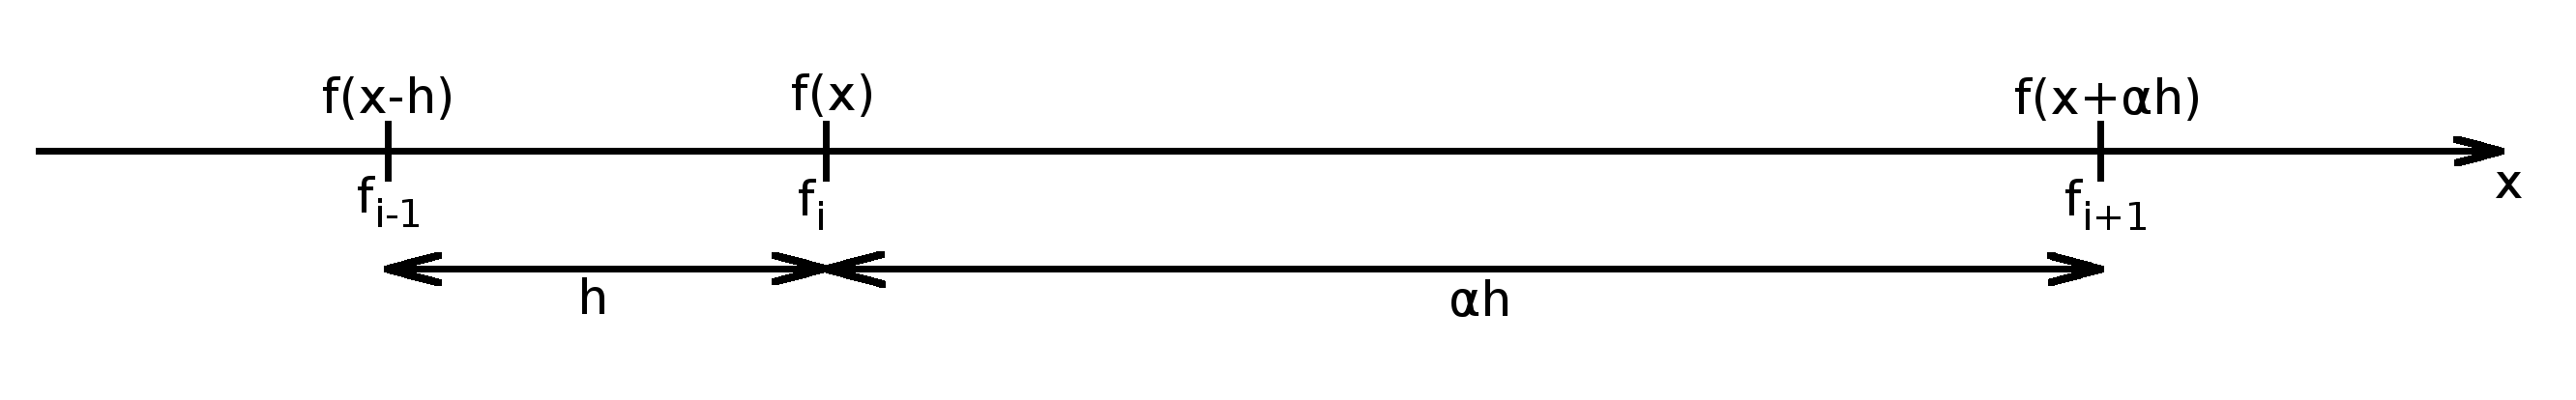
\includegraphics[width=1.\textwidth]{/home/argo/masterarbeit/thesis/images/2nd_derivative_2-point_formula_illustration.png}
	\caption{Function $f(x)$ and its discretization $f_i$ on a non-equidistant grid.}
	\label{fig:2_point_formula_illustration}
\end{figure}


For simplicity we restricted the function argument $x \in \mathcal{R}$. In the case $x \in \mathcal{R}^n$ the Jacobian is gained by performing directional derivatives. So e.g. for the one-sided first derivative $n+1$ function evaluations are necessary. \\

The great advantage of finite differences are their simple implementation. We can treat the (arbitrarily elaborate) function as a black box, perturb the input arguments a bit, perform $n+1$ function evaluations and get an approximation of the derivative. \\
This simplicity is at the expense of accuracy. If we choose $h$ too small, cancellation occurs. Otherwise with $h$ large the remainder term of the Taylor expansion gets large as well. So there exist an optimal $h$ to minimize the error although then the derivative approximation is still not exact.




\subsubsection{Automatic Differentiation and Internal Numerical Differentiation}
The basic idea of Automatic Differentiation (AD) is to subdivide a function $f: \mathcal{R}^n \rightarrow \mathcal{R}^m$ into so called elementary functions $\varphi_i$ from which the derivative is known. 

The evaluation of these elementary functions give intermediate values $v_i = \varphi(v_j)_{j \prec i}$ where the dependency relation $\prec$ is defined as

\begin{equation}
j \prec i \Leftrightarrow v_j \text{\textit{ is an argument of }} \varphi_i.
\end{equation}

By successively applying the chain rule one obtains the derivative of $f$.
One can distinguish the forward and reverse mode which will be explained in more detail now and exemplified by means of the example function

\begin{equation}
F(x) = 
\begin{bmatrix}
\exp((1+x_1)^2) + x_3 \\
x_2 \cdot \sin(1+x_1)
\end{bmatrix}
\end{equation}

\todo{Graph mit den einzelnen Berechnungsverzweigungen noch einfuegen?}

\paragraph{Forward Mode}\mbox{}\\
In the forward mode the directional derivative $\dot{y}$ is computed for a given direction in the function arguments $\dot{x}$ at a evaluation point $x$:

\begin{equation}
\dot{y} = \frac{\partial f}{\partial x}(x) \cdot \dot{x}
\label{eq:AD_example}
\end{equation}

The algorithm called first order forward sweep is structured into three parts. First the auxiliary variables $v_{1-n},...,v_0$ and $\dot{v}_{1-n},...,\dot{v}_0$ are initialized with the evaluation point $x$ and the direction of the directional derivative $\dot{x}$. So if we want to get $\frac{\partial f}{\partial x_2}$ we would need to set $\dot{x} = \begin{bmatrix}
0 & 1 & 0 & \dots & 0
\end{bmatrix}^T$. One can see here that with one forward sweep we get one column of the Jacobian $ \frac{\partial f}{\partial x}$. 
After the initialization the actual forward sweep begins where the $k$ elemental functions of $f$ are evaluated and saved in the intermediate values $v_i$. Simultaneously their derivatives  $\dot{v}_i$ are computed using previously calculated intermediate values. E.g. for $v_2 = \varphi_2(v_0, v_1)$ it would hold $\dot{v}_2 = \frac{\partial \varphi_2}{\partial v_0} \dot{v_0} + \frac{\partial \varphi_2}{\partial v_1} \dot{v_1}$. \\
The last $m$ intermediate variables represent the solution vector. So finally this values and derivatives are extracted.


\todo{Q: Ist das hier eine totale Ableitung?}


\begin{table}[H]
	\begin{tabular}{|c | l c l | l |} \hline
		Initialization & $[v_{i-n}, \dot{v}_{i-n}]$ & $=$ & $[x_i, \dot{x}_i]$ & $i=1,...,n$ \\ \hline
		Intermediate steps & $[v_{i}, \dot{v}_{i}]$ & $=$ & $[\varphi_i(v_j)_{j \prec i}, \sum_{j \prec i} \frac{\partial \varphi_i}{\partial v_j}(v_j) \cdot \dot{v}_j]$ & $i=1,...,k$ \\ \hline
		Extract solution & $[y_{m-i}, \dot{y}_{m-i}]$ & $=$ & $[v_{k-i}, \dot{v}_{k-i}]$ & $i=m-1,...,0$ \\ \hline
	\end{tabular}
	\caption{First order forward sweep}
	\label{tab:first_order_forward_sweep}
\end{table}

In order to illustrate this algorithm we will apply it onto the example function \eqref{eq:AD_example}:

\begin{table}[H]
	\centering
	\begin{tabular}{| c | l | l |} \hline
		Initialization & $v_{-2} = x_1$ & $\dot{v}_{-2} = \dot{x_1}$ \\
		& $v_{-1} = x_2$ & $\dot{v}_{-1} = \dot{x}_2$ \\
		& $v_{0} = x_3$ & $\dot{v_{0}} = \dot{x}_3$ \\ \hline
		Intermediate Steps & $v_1 = 1+v_{-2}$ & $\dot{v_1} = 1 \cdot \dot{v}_{-2}$ \\
		& $v_2 = v_{1}^2$ & $\dot{v_2} = 2 v_1 \cdot \dot{v}_{1}$ \\
		& $v_3 = \exp(v_{2})$ & $\dot{v_3} = \exp(v_2) \cdot \dot{v}_{2}$ \\
		& $v_4 = \sin(v_{1})$ & $\dot{v_4} = \cos(v_1) \cdot \dot{v}_{1}$ \\
		& $v_{5} = v_3 + v_0$ & $\dot{v_{5}} = 1 \cdot \dot{v}_3 + 1 \cdot \dot{v}_0$ \\
		& $v_{6} = v_{-1} + v_4$ & $\dot{v_{6}} = v_4 \cdot \dot{v}_{-1} + v_4 \cdot \dot{v}_{-1}$ \\ \hline
		Extract  solution & $y_1 = v_5$ & $\dot{y}_1 = \dot{v}_5$ \\
		& $y_2 = v_6$ & $\dot{y}_2 = \dot{v}_6$ \\ \hline
	\end{tabular}
	\caption{First order forward sweep applied on \eqref{eq:AD_example}.}
\end{table}




\paragraph{Adjoint Mode}\mbox{}\\
Beside the forward mode there is the adjoint mode where the adjoint directional derivative $\bar{x}^T$ is computed for a given adjoint direction $\bar{y}^T$ at the evaluation point $x$. 

\begin{equation}
\bar{x}^T = \bar{y}^T \frac{\partial f}{\partial x}(x)
\end{equation}

The algorithm is shown in Table \ref{tab:first_order_adjoint_sweep}. In contrary to the forward mode we need here an additional set of adjoint intermediate variables $\bar{v}_i$. These contain the adjoint sensitivity information which are initialized to zero in the first step. \\
The following forward sweep is analog to the one shown in Table \ref{tab:first_order_forward_sweep}, however here we compute just the intermediate function evaluations without derivatives. We need these function values in the next part. \\
The actual adjoint directional derivatives are now computed in the reverse sweep which consists of three sub-steps. First of all the adjoint directions $\bar{y}$ is chosen. So for example, if we want the second row of the Jacobian $\frac{\partial f_2}{\partial x}$ we need to set $\bar{y} = \begin{bmatrix}
0 & 1 & 0 & \dots & 0
\end{bmatrix}^T$.
Next all contributions to the adjoint intermediate variables will be successively summed up by applying the adjoint equation $\bar{y}^T \dot{y} = \bar{y}^T J \dot{x} = \bar{x}^T \dot{x}$ in a reverse scheme (that is why we need the forward sweep and hence the intermediate value evaluations first). Finally we can extract the solution $\bar{x}$ which corresponds to a row in $\frac{\partial f}{\partial x}$.


\begin{table}[H]
	\centering
	\begin{tabular}{| c | l c l | l |} \hline
		Initialization & $\bar{v}_i$ & $=$ & $0$ & $i=1-n,...,k-m$ \\ \hline
		& $v_{i-n}$ & $=$ & $x_i$ & $i=1,...,n$ \\
		Forward Sweep & $v_{i}$ & $=$ & $\varphi_i(v_j)_{j \prec i}$ & $i=1,...,k$ \\
		& $y_{m-i}$ & $=$ & $v_{k-i}$ & $i=m-1,...,0$ \\ \hline
		& $\bar{v}_{k-i}$ & $=$ & $\bar{y}_{m-i}$ & $i=0,...,m-1$ \\
		Reverse Sweep & $\bar{v}_j$ & $+ \hspace{-0.1cm} =$ & $\bar{v}_i \frac{\partial \varphi_i}{\partial v_j}(v_j) \quad \forall \ j \prec i$ & $i=k,...,1$ \\
		& $\bar{x}_i$ & $=$ & $\bar{v}_{i-n}$ & $i=n,...,1$ \\ \hline
	\end{tabular}
	\caption{First order adjoint sweep}
	\label{tab:first_order_adjoint_sweep}
\end{table}

Again we apply this algorithm on the exemplary function \eqref{eq:AD_example}:

\begin{table}[H]
	\centering
	\begin{tabular}{| c | l | l |} \hline
		Initializiation & $\bar{v}_{-2}=\dots=\bar{v}_4=0$ & \\ \hline
		& \textbf{Forward Sweep} & \textbf{Reverse Sweep} \\ \hline
		Initialization & $v_{-2}=x_1$ & $\bar{v}_6=\bar{y}_2$ \\
		& $v_{-1}=x_2$ & $\bar{v}_5=\bar{y}_1$ \\
		& $v_{0}=x_3$ &  \\	\hline
		Sweep & $v_1=1+v_{-2}$ & $\bar{v}_{-1} +\hspace{-0.1cm}= \bar{v}_6 \cdot v_4$ \\
		& $v_2=v_{1}^2$ & $\bar{v}_{4} +\hspace{-0.1cm}= \bar{v}_6 \cdot v_{-1} $ \\
		& $v_3=\exp(v_2)$ & $\bar{v}_{3} +\hspace{-0.1cm}= \bar{v}_5 \cdot 1 $ \\
		& $v_4= \sin(v_1)$ & $\bar{v}_{0} +\hspace{-0.1cm}= \bar{v}_5 \cdot 1 $ \\
		& $v_5=v_{3} + v_0$ & $\bar{v}_{1} +\hspace{-0.1cm}= \bar{v}_4 \cdot \cos(v_1) $ \\
		& $v_6=v_{-1} \cdot v_4$ & $\bar{v}_{2} +\hspace{-0.1cm}= \bar{v}_3 \cdot \exp(v_2) $ \\
		& & $\bar{v_1} +\hspace{-0.1cm}= \bar{v}_2 \cdot 2 v_1$ \\
		& & $\bar{v_{-2}} +\hspace{-0.1cm}= \bar{v}_1 \cdot 1$	\\ \hline
		Extract solution & $y_1 = v_5$ & $\bar{x}_3 = \bar{v}_0$ \\
		& $y_2 = v_6$ & $\bar{x}_2 = \bar{v}_{-1}$ \\
		& & $\bar{x}_1 = \bar{v}_{-2}$	\\ \hline
	\end{tabular}
	\caption{First order adjoint sweep applied on \eqref{eq:AD_example}}
\end{table} 


Until now the fundamental principles of AD have been explained, i.e. just the first order derivative in forward and adjoint mode. Higher derivatives of arbitrary order can be obtained by using the method of Taylor coefficient propagation which is based on the propagation of a Taylor polynomial through a function evaluation. The higher derivatives can then be extracted by scaling of the polynomial coefficients. \\

In this thesis we are actually interested in the sensitivities $\frac{\partial y}{\partial p}$ of an differential equation $\dot{y}=f(t,y;p)$ with respect to parameters $p$. The application of AD on differential equations is called Internal Numerical Differentiation (IND). The principle is based on the fact that solving numerically a differential equation consists of many elemental operations from which the derivatives are known. So it is straight forward to apply the chain rule on all these elemental operations in order to get the derivative $\frac{\partial y}{\partial p}$ just as explained above. \\
A detailed explanation on taylor coefficient propagation for higher derivatives and IND can be found in \cite{diss_jan}. \todo{Reicht das... mehr?}



\subsection{Numerical solution of initial value problems (IVP)}
In this section numerical methods will be introduced to solve initial value problems of the form

\begin{align}
	\dot{x} & = f(t,x(t)) \\
	x(t_0) & = x_0 \nonumber
\end{align}

where $t_0$ is the initial time and $x_0$ the initial value. \\

There are a lot of different numerical methods like explicit/implicit Euler, Runge-Kutta (RK) or linear multistep methods (LMM). The solver we used in this thesis applies the method of Backward Differentiation Formulas (BDF) which will be explained further now.

The basic idea of the BDF method of order $k$ is to interpolate the last $(k+1)$ solution points $x_m,...,x_{m+k}$ with an polynomial such that the unknown point $x_{m+k}$ satisfies the ODE at $t_{m+k}$. 
It is defined as

\begin{equation}
	\sum_{i=0}^{k} \alpha_{im} x_{m+i} = h_{m+k-1} f(t_{m+k},x_{m+k})
	\label{eq:bdf_formula}
\end{equation}

where $\alpha \in \mathbb{R}$, $\alpha_{0m},\alpha_{km} \ne 0 \ \forall \ m$ are the coefficients which can be computed by multiplying the step width with the derivative of the interpolation polynomial.  \\
BDF methods up to order 6 are used in practice because these are zero-stable \cite{numerik1_skript_koerkel}. \\
Since \eqref{eq:bdf_formula} is a non-linear system of equations it is solved iteratively using Newton's method. In order to obtain a good starting point a so called predictor is used, which is the integration polynomial of the previous integration step. With this initial guess for $x_{m+k}$ the Newton method can be applied to get the so called corrector polynomial, which satisfies the differential equation at $t_{m+k}$. \\
As we want the numerical integrator both to perform large integration steps to minimize the required time to solve the IVP and limit the inevitable numerical errors on a predefined value we are dependent on a strategy to choose the step width $h_{m+k-1}$ accordingly. This is done by estimating the local error in each integration step. Either the local error is smaller than some tolerance then the step width will be increased, otherwise decreased until the local error tolerance is satisfied. \\







\subsection{PDE discretization: Method of lines}
\label{subsection:pde_discretization}



Given a partial differential equation (PDE) in the differential variable $u(t,x)$ (e.g. temperature dependent on time $t \in \mathbb{R}$ and space coordinate $x \in \Omega \subseteq \mathbb{R}^D$ with $D=\{1,2,3\}$). The method of lines is used to discretize the PDE in space such that with $N$ discretization points we get $N$ differential variables only dependent in time:

\begin{equation}
	u(x,t) \ \rightarrow \ \{ u_0(t), u_1(t), ..., u_{N-1}(t) \}
\end{equation}

This is illustrated in Fig. \ref{fig:pde_discretization_method_of_lines} in one space dimension $x$ at time $\hat{t}$.

\begin{figure}[H]
	\centering
	\begin{tikzpicture}
	\begin{axis}[domain=-1:6.3,
	samples=100,
	ymin=0, ymax=5	,	
	xmin=-1, xmax=8,	 
	axis lines=left,
	xtick={2, 4},
	xticklabels={$x_i$, $x_{i+1}$},
	ytick=\empty,
	xlabel=$x$, xlabel style={at=(current axis.right of origin), anchor=west},
	ylabel=\empty
	]
	
	\addplot+[color=black, mark=none] {0.7*cos(deg(x)) + 3}
	node[pos=1.1] {$u(x,\hat{t})$};
	\addplot[only marks, mark=*, color=black] 
	table {0 3.7
		1 3.37
		2 2.7
		4 2.55
		5 3.2
	}
	node[above, pos=0.55] {$u_i(\hat{t})$}
	node[above, pos=0.7] {$u_{i+1}(\hat{t})$}; 
	\end{axis}
	\end{tikzpicture}
	\caption{Spatial discretization of $u(x,t)$ with discretization points $x_i$ and $h_i:=x_{i+1} - x_i$}
	\label{fig:pde_discretization_method_of_lines}
\end{figure}


Spatial derivatives within the PDE are approximated using the finite difference formulas derived in section \ref{subsubsec:finite_differences}. \\
The differential variables $u_i$ of the resulting system are then just dependent on time $t$ such that we have an ODE system now. The PDE's boundary conditions (BC) are applied by using the differential variables at the border, in the 1D case this would be obviously $u_0$ and $u_{N-1}$. \\
Dirichlet boundary conditions 
\begin{equation}
u(x_0, t) = u_0^{BC}(t)
\end{equation}

which fix the function value are applied by

\begin{align}
	u_0(t) & = u_0^{BC}(t) \\
	\Leftrightarrow \dot{u}_0(t) & = \dot{u}_0^{BC}(t) \nonumber
\end{align}

On the other hand Neumann boundary conditions

\begin{equation}
	\nabla u(x_{0},t) = J_u
\end{equation}

setting the flux into the spatial domain $\Omega$ to a certain value

\begin{align}
	\frac{u_{1} - u_{0}}{x_{1} - x_{0}} = J_u  \\
	\Leftrightarrow u_0 = u_1 + J_u (x_1 - x_0) \nonumber
\end{align}

The function value of $u_0$ is already defined by $u_1$ so $\dot{u}_0$ is not necessary.




\subsection{Optimization Task: Parameter Estimation}
%In this section we treat the least squares problem of the form
%
%\begin{align}
%	\min_{x(t),p} \ & \frac{1}{2} ||F(x(t;x_0,p),p)||_2^2 \\
%	s.t. \quad & \dot{x} = f(x,t;p) \quad \forall t \in [t_0, t_f] \nonumber \\
%	& x(0) = x_0 \nonumber
%\end{align}
%
%where $F \in \mathbb{R}^{n_{MP}}$ is the residuum vector of the measurement points, $x \in \mathbb{R}^{n_x}$ are the differential variables satisfying the embedded initial value problem and $p \in \mathbb{R}^{n_p}$ are the parameters being optimized. \\
%\todo{Frage ist ob man es sehr allgemein erklaert mit NOC und SOC von sehr allgemeinem gleichungsbeschraenken Optimierungsproblem. Oder aber eher fuer uns relevanten Fall von least squares problemen und Loesung dann mit Gauss-Newton. Problem ist das wir momentan gar kein Gauss-Newton Verfahren benutzen... fragen!!}

\subsubsection{General NLP and optimality criterions}
In this section we first treat the general nonlinear optimization problem (NLP) of the form

\begin{align}
	\min_x & \ f(x) \label{eq:NLP_formulation} \\
	s.t. & \ g(x) = 0 \nonumber \\
	& \ h(x) \ge 0 \nonumber
\end{align}

where $x \in \mathbb{R}^n$ is the optimization variable, $f: \mathbb{R}^n \rightarrow \mathbb{R}$ is the objective function, $g: \mathbb{R}^n \rightarrow \mathbb{R}^{m_2}$ and $h: \mathbb{R}^n \rightarrow \mathbb{R}^{m_3}$ are the equality and respectively inequality constraints. Index $m_1$ is missing because we will need this later in the context of the least squares problem. \\
The corresponding Lagrange function of \eqref{eq:NLP_formulation} is defined as

\begin{equation}
	\mathcal{L}(x,\lambda,\mu) := f(x) - \lambda^T g(x) - \mu^T h(x)
\end{equation}

with Lagrange multipliers $\lambda \in \mathbb{R}^{m_2}$ and $\mu \in \mathbb{R}^{m_3}$. \\

Before stating the major results from optimization theory we need to introduce the following definitions:

\begin{Definition}
	$S = \{ x \ | \ g(x) = 0 \ \text{and} \ h(x) \ge 0 \}$ is called \underline{feasible set}.
\end{Definition}

\begin{Definition}
	$I(x) = \{ i=1,...,m_3 \ | \ h(x) = 0 \}$ is called \underline{active set} with $s := \vert I \vert$.
\end{Definition}

\begin{Definition}
	$\tilde{g}(x) := 
	\begin{pmatrix}
		g(x) \\
		h_i(x), \ i \in I(x) 
	\end{pmatrix}$
\end{Definition}

\begin{Definition}
	$x$ is called \underline{regular} if [LICQ] is satisfied, i.e. $rank \left( \frac{\partial \tilde g(x)}{\partial x} \right) = m_2 + s$
\end{Definition}

\begin{Definition}
	\textbf{(Tangent space)} \\
	$T(x) = \left\{ p \in \mathbb{R}^n \ | \ \frac{\partial \tilde g(x)}{\partial x} \cdot p = 0 \right\}$ \\
	$T^+(x) = \left\{ p \in \mathbb{R}^n \ | \ \frac{\partial g(x)}{\partial x} \cdot p = 0, \frac{\partial h_i(x)}{\partial x} \cdot p = 0 \text{ and } \mu_i > 0 \text{ for } i \in I(x) \right\}$ \\
	are called \underline{tangent space}. It holds $T(x) \subseteq T^+(x)$.
\end{Definition}



Major results from optimization theory are the necessary optimality condition [NOC] and sufficient optimality condition [SOC]: 

\begin{Theorem}
	$[\text{\textbf{NOC}}]$ \\
	Let $x^*$ be a local minimum and regular, then
	\begin{enumerate}
		\item $\exists \lambda^* \in \mathbb{R}^{m_2}, \mu^* \in \mathbb{R}^{m_3}, \mu^* \ge 0$ s.t. \\
		$\nabla_x \mathcal{L}(x^*, \lambda^*, \mu^*) = 0$ and \\
		$(\mu^*)^T \cdot h(x^*) = 0$ complementary condition [CC]
		\item $p^T \nabla_x^2 \mathcal{L}(x^*, \lambda^*, \mu^*) p \ge 0 \ \forall \ p \in T(x^*)$
	\end{enumerate}
\end{Theorem}


\begin{Theorem}
	$[\text{\textbf{SOC}}]$ \\
	Let $x^* \in S$ and let there exist $\lambda^*, \mu^* \ge 0$ such that $\nabla_x \mathcal{L}(x^*, \lambda^*, \mu^*) = 0$ and \\ $(\mu^*)^T \cdot h(x^*) = 0$. 
	Let $p^T \mathcal{L}(x^*, \lambda^*, \mu^*) p > 0$ for $p \in T^+(x^*) \backslash \{0\}$. \\
	Then: $x^*$ is a strict local minimum.
\end{Theorem}

\todo{KKT conditions einfuehren!} \\

\subsubsection{Non-linear least squares problem and Gauss-Newton method}
Since we are performing a parameter estimation we will treat now an equality constrained nonlinear least squares problem

\begin{align}
	\min_x \ & || F_1(x) ||_2^2 \\
	s.t. \ & F_2(x) = 0 \nonumber
\end{align}

with $x \in \mathbb{R}^n$, $F_1: \mathbb{R}^n \rightarrow \mathbb{R}^{m_1}$ and $F_2: \mathbb{R}^n \rightarrow \mathbb{R}^{m_2}$. Inequality constraints will be introduced in the context of the Active Set Strategy (ASS) later. \\
Instead of applying the KKT conditions on this problem we first linearize in order to avoid the need of computing the Hessian. This method is called Gauss-Newton (GN) and the resulting problem reads as

\begin{align}
\min_{\Delta x} \ & || F_1(x) + J_1(x) \Delta x ||_2^2 \\
s.t. \ & F_2(x) + J_2(x) \Delta x = 0 \nonumber
\end{align}

with $J_1(x) = \frac{\partial F_1(x)}{\partial x} \in \mathbb{R}^{m_1 \times n}$ and $J_2(x) = \frac{\partial F_2(x)}{\partial x} \in \mathbb{R}^{m_2 \times n}$. Applying the KKT conditions on this system gives the system

\begin{equation}
	\begin{bmatrix}
		J_1^T J_1 & -J_2^T \\
		J_2 & 0
	\end{bmatrix}
	\begin{bmatrix}
		\Delta x \\
		\lambda
	\end{bmatrix}
	= -
	\begin{bmatrix}
	J_1^T F_1 \\
	F_2
	\end{bmatrix}
	\label{eq:GN_KKT_system}
\end{equation}


An important result is

\begin{Lemma} \textcolor{white}{.}\\
	If $rank(J_2) = m_2$ and $rank 
	\begin{pmatrix}
	J_1 \\
	J_2
	\end{pmatrix}
	= n$,
	then 	
	$\begin{pmatrix}
		J_1^T J_1 & -J_2^T \\
		J_2 & 0
	\end{pmatrix}$
	is non-singular.
\end{Lemma}

\subsubsection{Numerical solution}
For the numerical solution of \eqref{eq:GN_KKT_system} we will successively introduce the unconstrained, the equality constrained and the general equality and inequality constrained case because they are built up on each other.

\paragraph{Unconstrained case}\mbox{}\\
In the unconstrained case we want to solve the problem

\begin{equation}
\min_{\Delta x} \frac{1}{2} || F_1 + J_1 \Delta x ||_2^2
\label{eq:numerical_solution_LSQ}
\end{equation}

Based on decomposing $J_1$ two solutions are shown:

\begin{itemize}
	\item \textbf{QR decomposition} \\
	First we decompose $J_1$
	\begin{equation}
		J_1 = Q R = 
		\begin{pmatrix}
			Q1 & Q2
		\end{pmatrix}
		\begin{pmatrix}
			\bar{R} \\
			0
		\end{pmatrix}
	\end{equation}
	where $Q$ is an orthogonal matrix and $\bar{R}$ is an upper triangular matrix. Inserting in the objective function \eqref{eq:numerical_solution_LSQ} gives
	
	\begin{align}
		|| F_1 + J_1 \Delta x ||_2^2 & = || F_1 + Q R \Delta x ||_2^2 = || Q( Q^T F_1 + R \Delta x ||_2^2 \\
		& = \left| \left| \begin{pmatrix}
		Q_1^T F_1 \\
		Q_2^T F_1
		\end{pmatrix} + 
		\begin{pmatrix}
		\bar{R} \\
		0
		\end{pmatrix}
		\Delta x \right| \right|_2^2 \nonumber \\
		& = || Q_1^T F_1 + \bar{R} \Delta x ||_2^2 + ||Q_2^T F_1 ||_2^2 \nonumber
	\end{align}
	
	If $rank(J_1)=n$ and therefore $\bar{R}$ invertible one can solve for $\Delta x$ easily because $\bar{R}$ is triangular:
	
	\begin{equation}
		\bar{R} \Delta x = -Q_1^T F_1
	\end{equation}
	
	\item \textbf{Singular value decomposition (SVD)} \\
	Using SVD $J_1$ decomposes to
	\begin{equation}
		J_1 = U \Sigma V^T =
		\begin{pmatrix}
			U_1 & U_2
		\end{pmatrix}
		\begin{pmatrix}
			\bar{\Sigma} \\
			0
		\end{pmatrix}
		\begin{pmatrix}
			V_1 \\
			V_2
		\end{pmatrix}
	\end{equation}
	
	with $U, V$ orthogonal and $\bar{\Sigma}$ diagonal. Let $r := rank(J_1) \le n$. Then $\bar{\Sigma}$ has the singular values $\sigma_1 \ge \sigma_2 \ge ... \ge \sigma_r > 0 > ... > 0$ on the diagonal. \\
	Inserting modifies \eqref{eq:numerical_solution_LSQ} by
	
	\begin{align}
		|| F_1 + J_1 \Delta x ||_2^2 & = || F_1 + U \Sigma \overbrace{V^T \Delta x}^{=: \Delta y} ||_2^2 = || U ( U^T F_1 + \Sigma \Delta y ||_2^2 \label{eq:numerical_solution_LSQ_SVD} \\
		& = \left| \left| \begin{pmatrix}
		U_1^T F_1 \\
		U_2^T F_1
		\end{pmatrix} + 
		\begin{pmatrix}
		\bar{\Sigma} \\
		0
		\end{pmatrix}
		\Delta y \right| \right|_2^2 \nonumber \\
		& = || \underbrace{U_1^T F_1}_{=: c} + \bar{\Sigma} \Delta y ||_2^2 + || U_2^T F_1 ||_2^2 \nonumber
	\end{align}
	
	For $rank(J_1) < n$ the solution $\Delta y$ is not unique to minimize \eqref{eq:numerical_solution_LSQ_SVD}. By choosing
	
	\begin{align}
		\Delta y_i = 
		\begin{cases}
			- \frac{c_i}{\sigma_i} \ & \text{for } i=1,...,r \\
			\ 0 \ & \text{else}
		\end{cases}
	\end{align}
	
	we get the final result $\Delta x$ with
	
	\begin{equation}
		\Delta x = V \Delta y
	\end{equation}
	
	\todo{Lemma von ODE Skript noch rein?}

\end{itemize}


\paragraph{Equality constrained case}\mbox{}\\
In the equality constrained case we handle the problem

\begin{align}
	\min_{\Delta x} & \ \frac{1}{2} || F_1 + J_1 \Delta x ||_2^2 \label{eq:numerical_soln_eq_constrained_LSQ} \\
	s.t. & \ F_2 + J_2 \Delta x = 0 \nonumber
\end{align}

For the case $rank(J_2)=m_2$ we will use a QR decomposition:

\begin{equation}
	J_2^T = Q R = 
	\begin{pmatrix}
		Q_1 & Q_2
	\end{pmatrix}
	\begin{pmatrix}
		\bar{R} \\
		0
	\end{pmatrix}
\end{equation}

Inserting into the equality constraint gives

\begin{equation}
	F_2 + J_2 \Delta x = F_2 + R^T \overbrace{Q^T \Delta x}^{=: \Delta y} = F_2 +
	\begin{pmatrix}
		\bar{R}^T & 0
	\end{pmatrix} 
	\begin{pmatrix}
		\Delta y_1 \\
		\Delta y_2
	\end{pmatrix} = F_2 + \bar{R}^T \Delta y_1 = 0
\end{equation}

Since $rank(J_2)=m$, $\bar{R}^T$ is invertible and we can solve for $\Delta y_1$ because $\bar{R}^T$ is triangular:

\begin{equation}
	\bar{R}^T \Delta y_1 = -F_2
\end{equation}

With the solution $\Delta y_1^*$, recalling $\Delta x = Q \Delta y$ and the definition $J_1 Q = \begin{pmatrix} A_1 & A_2 \end{pmatrix}$ it remains to solve

\begin{align}
	\min_{\Delta y_2} \ \frac{1}{2} || (F_1 + A_1 \Delta y_1^*) + A_2 \Delta y_2 ||_2^2
\end{align}

which is an unconstrained least squares problem we discussed before. At last we need to compute $\Delta x = Q \Delta y$ for the final solution of \eqref{eq:numerical_soln_eq_constrained_LSQ}. \\
If $rank(J_2) < m_2$ one can perform a singular value decomposition of $J_2$ analog to the unconstrained case. \todo{stimmt das?}

\paragraph{Equality and inequality constrained case using active set strategy}\mbox{}\\
\begin{align}
\min_{\Delta x} & \ \frac{1}{2} || F_1 + J_1 \Delta x ||_2^2 \label{eq:numerical_soln_ineq_constrained_LSQ} \\
s.t. & \ F_2 + J_2 \Delta x = 0 \nonumber \\
&  \ F_3 + J_3 \Delta x \ge 0 \nonumber
\end{align}

Active Set Strategy algorithm:
\begin{enumerate}
	\item Choose start point $x^0$, set iteration number $k=0$ and check for feasibility of $x^0$ and compute  initial active set $I^0 = \{ i \ | \ F_3^i(x^0) = 0 \}$
	\item Compute extended equality constraints $\tilde{F}_2(x) = 
	\begin{pmatrix} 
	F_2(x) \\  
	F_3^i(x), \ i \in I^k
	\end{pmatrix}$
	\item Solve the extended equality constrained subproblem
	\begin{align}
		\min_{\Delta x} & \ \frac{1}{2} || F_1 + J_1 \Delta x ||_2^2 \nonumber \\
		s.t. & \ \tilde{F}_2 + \tilde{J}_2 \Delta x = 0 \nonumber
	\end{align}
	\item Check for constraint violations $F_3(x^k + \Delta x^k) < 0$, modify $\Delta x^k$ such that $x^{k+1}$ is feasible and add corresponding constraints to active set.
	\item Compute $x^{k+1} = x^k + t^k \Delta x^k$ with stepsize $t^k \in (0, 1]$ from linesearch algorithm.
	\item Compute Lagrange multiplier $\mu$ from active inequality constraints and remove from active set if $\mu_i < 0$.
	\item Set $x^k = x^{k+1}$, $k += 1$ and goto step 2.
\end{enumerate}



\newpage
\section{Simulation of DSC measuring process}
\subsection{Mathematical model}

Our 1D mathematical model is based on the following assumptions. First the heat transport is exclusively done by thermal diffusion (c.f. section \ref{sec:heat_equation}, equation \eqref{eq:heat_equation}), so convection and thermal radiation are neglected. Furthermore the mass density $\rho$ and heat conductivity $\lambda$ of the PCM are constant.

\begin{equation}
\rho c_p(T(x,t)) \frac{\partial T}{\partial t}(x,t) = \nabla \cdot \left[\lambda \cdot \nabla T(x,t)  \right]
\label{eq:heat_equation}
\end{equation}

Moreover we assume that the reference and sample crucible (see Fig. \ref{fig:heat_flux_DSC}) are independent of each other which allows us to simulate each side on its own. 

\begin{figure}[H]
	\centering
	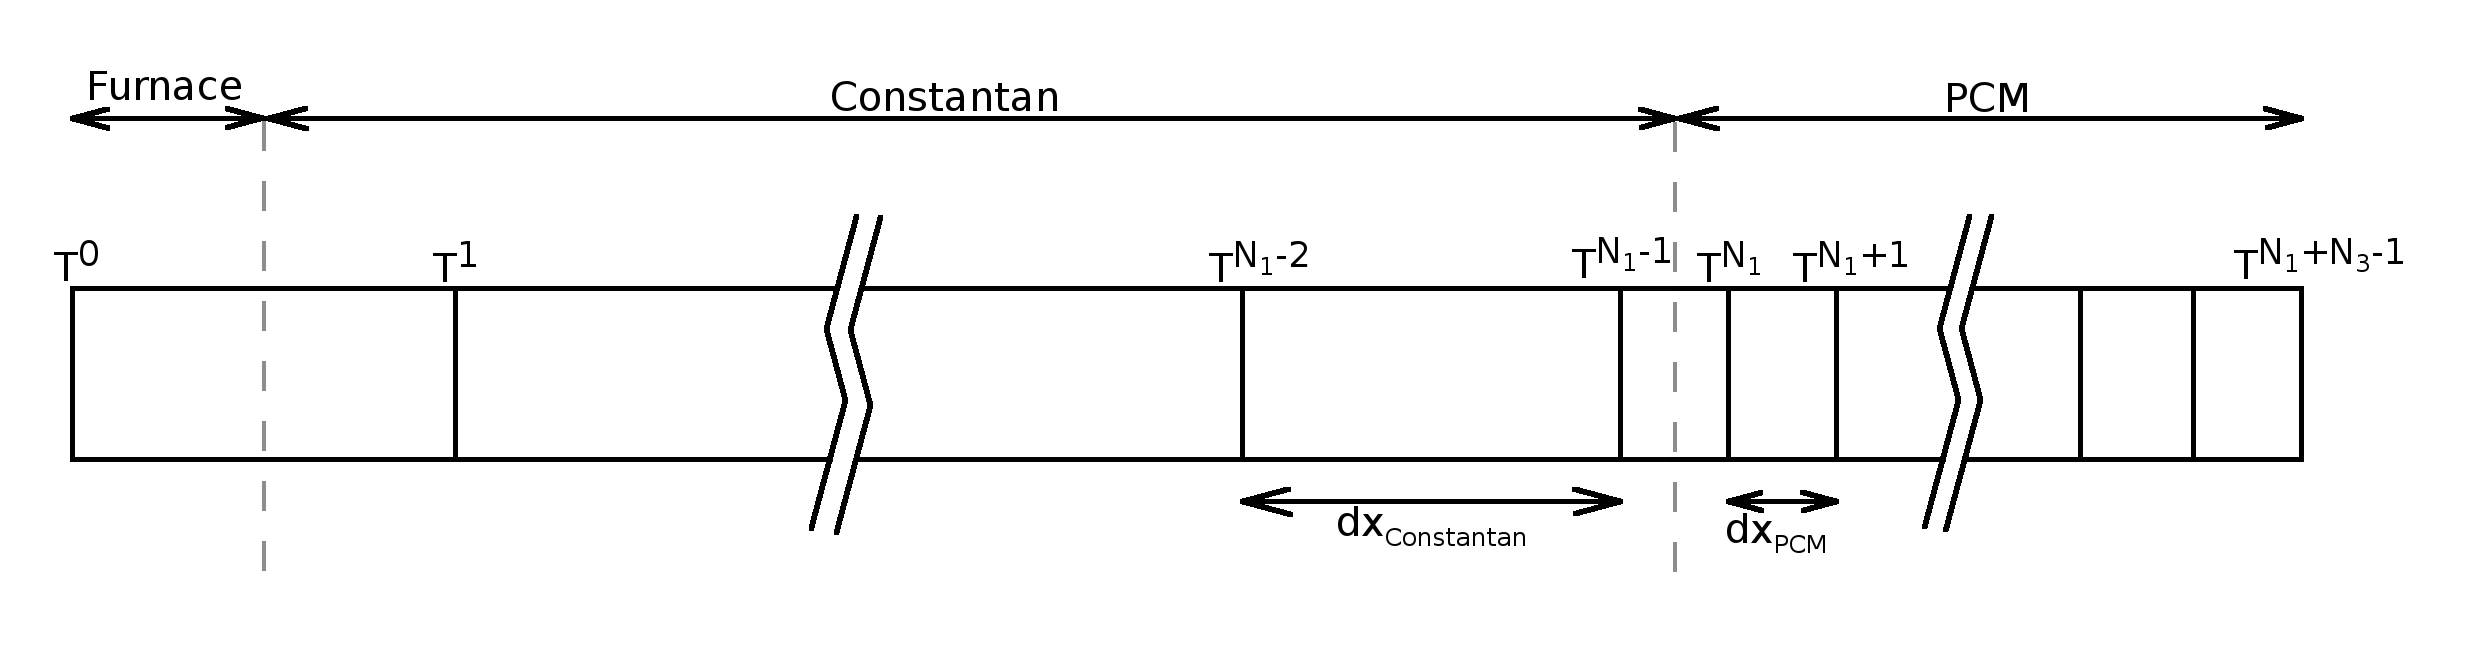
\includegraphics[width=1.\textwidth]{/home/argo/masterarbeit/vortrag/images/discretization_grid.png}
	\caption{}
	\label{fig:mathematical_model_discretized}
\end{figure}

Correspondingly in Fig. \ref{fig:mathematical_model_discretized} one can see the spatially discretized model of the sample side, where on the very left is the furnace. Heat then flows through the silver plate finally into the PCM. Since the furnace is heated in such a way by regulating that the temperature at the reference crucible increases linearly with a heating rate $\beta$ and due to constant material properties of silver with respect to temperature the furnace' temperature increases as well with a constant rate $\beta$. From this follows the first boundary condition

\begin{equation}
	T^0 = T_0 + \beta t
\end{equation}

with a start temperature $T_0$ and the heating rate $\beta$. For the boundary condition at the right hand side we assume that no heat can leave the PCM. So the heat flux is

\begin{equation}
	\Phi_q^{N-1} = \lambda_{pcm} \frac{T^N - T^{N-1}}{\Delta x^N} = 0
\end{equation}

using Fourier's law and a virtual grid point $T^N$. \\
At time $t_0=0$ we assume that the temperature is equal everywhere:

\begin{equation}
	T^i(t_0=0) = T_0 \ \forall \ i \in \{ 0,1,...,N-1 \}
\end{equation}

For the spatial discretization of the heat equation we applied the method of lines. Since the heat conductivity $\lambda$ is constant everywhere, on the RHS of heat equation \eqref{eq:heat_equation} is a second derivative with respect to space. For the discretization on a non-homogeneous grid we used equation \eqref{eq:2_point_formula_inhomogeneous}. The resulting system of ordinary differential equations is given by

\begin{align}
\hspace{-1cm}
\frac{d}{dt} \begin{bmatrix*}
T^0 \\[1ex]
T^1 \\[0.3ex]
\vdots \\[1ex]
T^{N_1-2} \\[1.7ex]
T^{N_1-1} \\[1.7ex]
T^{N_1} \\[0.5ex]
\vdots \\[1.5ex]
T^{N_1+N_3-2} \\[1ex]
T^{N_1+N_3-1}
\end{bmatrix*} =
\begin{bmatrix}
\beta \\
\frac{\lambda^{\text{Ag}}}{\rho^{\text{Ag}} \ c_p^{\text{Ag}}} \cdot \frac{T^{0} - 2 T^{1} + T^{2}}{\Delta x_{\text{Ag}}^2} \\
\vdots \\
\frac{\lambda^{\text{Ag}}}{\rho^{\text{Ag}} \ c_p^{\text{Ag}}} \cdot \frac{T^{N_1-3} - 2 T^{N_1-2} + T^{N_1-1}}{\Delta x_{\text{Ag}}^2} \\
\frac{\lambda^{\text{Ag}}}{\rho^{\text{Ag}} \ c_p^{\text{Ag}}} \cdot \frac{\frac{2}{1+\alpha} T^{N_1-2} - \frac{2}{\alpha} T^{N_1-1} + \frac{2}{\alpha (\alpha + 1)} T^{N_1}}{\Delta x_{\text{Ag}}^2} \\
\frac{\lambda^{\text{PCM}}}{\rho^{\text{PCM}} \ c_p^{\text{PCM}}(T^{N^1})} \cdot \frac{T^{N_1-1} - 2 T^{N_1} + T^{N_1+1}}{\Delta x_{\text{PCM}}^2} \\
\vdots \\
\frac{\lambda^{\text{PCM}}}{\rho^{\text{PCM}} \ c_p^{\text{PCM}}(T^{N^1+N^3-2})} \cdot \frac{T^{N_1+N_3-3} - 2 T^{N_1+N_3-2} + T^{N_1+N_3-1}}{\Delta x_{\text{PCM}}^2} \\
\frac{\lambda^{\text{PCM}}}{\rho^{\text{PCM}} \ c_p^{\text{PCM}}(T^{N^1+N^3-1})} \cdot \frac{T^{N_1+N_3-2} - T^{N_1+N_3-1}}{\Delta x_{\text{PCM}}^2}
\end{bmatrix}
\label{eq:heat_equation_discretized}
\end{align}

where \todo{ODE system noch aktualisieren und beschreibung der einzelnen Terme.}



\subsection{Spatial discretization grid}
At first the spatial discretization grid was constant in the silver and PCM respectively with grid sizes $\Delta x_{\text{Ag}} > \Delta x_{\text{PCM}}$ because only in PCM the phase transition occurs we are interested in. As for the silver plate we get appropriate results for the lengths $L1=40$ and $L3=0.1$ there is a big discontinuity in the grid size at the transition from silver to PCM. In order to avoid numerical problems the used framework of generating a continuous grid will be explained now. \\
In the following $x$ will denote the physical grid, $\tilde{x}$ the computation grid and $\chi(\tilde{x}) = x$ the corresponding mapping which is defined by its derivative

\begin{equation}
	\frac{\partial \chi(\tilde{x})}{\partial \tilde{x}} := \frac{\Delta \bar{x} - \Delta \underline{x}}{1 + e^{\gamma(\tilde{x} - b)}} + \Delta \underline{x}
\end{equation}

with the parameters $\Delta \underline{x}, \Delta \bar{x}$ as lower and upper bounds of the grid size. $\gamma$ defines the transition shape and $b$ the transition position on the computation grid. Since these parameters are quite counterintuitive they will be calculated with the following parameters:

\begin{itemize}
	\item $N \in \mathbb{N}$: total number of computation grid points.
	\item $n_{pcm} \in (0,1)$: Ratio of grid points for the PCM.
	\item $n_{tr} \in (0,1)$: Ratio of grid points for the transition.
	\item $n_{m} \in (0,1)$: Ratio of grid points: Margin to the PCM, where the transition is finished up to a threshold.
	\item $t < 1$: At grid point $N-N_{pcm}-N_m$, $\frac{\partial \chi(\tilde{x})}{\partial \tilde{x}}$ has finished the transition by $(100 \cdot t)\%$.
\end{itemize}

First of all, the ratios of grid points $n_i$ can be converted easily into absolute numbers with $N_i = N \cdot n_i$. The central position of the grid transition in the computation grid size is

\begin{equation}
	b = N - N_{pcm} - N_m - \frac{1}{2} m_{tr}
	\label{eq:spatial_grid_b}
\end{equation}

Furthermore we get $\gamma$ by

\begin{subequations}
\begin{align}
	\frac{\partial \chi}{\partial \tilde{x}}(\tilde{x}=N-N_{pcm}-N_m) = & \Delta \underline{x} + (\Delta \bar{x} - \Delta \underline{x}) \cdot (1-t) \\
	\Leftrightarrow \frac{\Delta \bar{x} - \Delta \underline{x}}{1 + e^{\gamma(N-N_{pcm}-N_m - b)}} + \Delta \underline{x} = & \Delta \underline{x} + (\Delta \bar{x} - \Delta \underline{x}) \cdot (1-t)  \\
	\stackrel{\eqref{eq:spatial_grid_b}}{\Leftrightarrow}  1 + e^{\gamma \frac{N_{tr}}{2}} = & \frac{1}{1 - t}  \\[2ex]
	\Leftrightarrow \gamma = \frac{2}{N \cdot n_{tr}} \ln(\frac{t}{1-t})
\end{align}
\end{subequations}

The remaining variables $\underline{x}$ and $\bar{x}$ we get by the condition that $T^{N_1-1}$ is at the physical grid position $L_1$

\begin{subequations}
	\begin{align}
	\sum_{i=0}^{N_1 - 2} \frac{\partial \chi}{\partial \tilde{x}}(i) = & L_1 \\
	\Leftrightarrow \sum_{i=0}^{N_1 - 2} \left[ \frac{\Delta \bar{x} - \Delta \underline{x}}{1 + e^{\gamma(i - b)}} + \Delta \underline{x} \right] = & L_1 \\
	\Leftrightarrow \underbrace{ \left[ \sum_{i=0}^{N_1 - 2} \frac{1}{1 + e^{\gamma(i - b)}} \right] }_{=: W_{11}} \cdot \Delta \bar{x} + \underbrace{\left[ N_1 - 1 - \sum_{i=0}^{N_1 - 2} \frac{1}{1 + e^{\gamma(i - b)}} \right]}_{=: W_{12}} \cdot \Delta \underline{x} = & L_1
	\end{align}
\end{subequations}

and $T^{N_1+N_3-1}$ is at the physical grid position $L_1+L_3$

\begin{subequations}
	\begin{align}
	\sum_{i=0}^{N_1 + N_3 - 2} \frac{\partial \chi}{\partial \tilde{x}}(i) = & L_1 + L_3 \\
	\Leftrightarrow \sum_{i=0}^{N_1 + N_3 - 2} \left[ \frac{\Delta \bar{x} - \Delta \underline{x}}{1 + e^{\gamma(i - b)}} + \Delta \underline{x} \right] = & L_1 + L_3 \\
	\Leftrightarrow \underbrace{ \left[ \sum_{i=0}^{N_1 + N_3 - 2} \frac{1}{1 + e^{\gamma(i - b)}} \right] }_{=: W_{21}} \cdot \Delta \bar{x} + \underbrace{ \left[ N_1 + N_3 - 1 - \sum_{i=0}^{N_1 + N_3 - 2} \frac{1}{1 + e^{\gamma(i - b)}} \right] }_{=: W_{22}} \cdot \Delta \underline{x} = & L_1 + L_3
	\end{align}
\end{subequations}

This gives the linear system

\begin{equation}
	\begin{bmatrix}
		W_{11} & W_{12} \\
		W_{21} & W_{22}
	\end{bmatrix}
	\begin{bmatrix}
		\Delta \bar{x} \\
		\Delta \underline{x}
	\end{bmatrix}
	= 
	\begin{bmatrix}
		L_1 \\
		L_1 + L_3
	\end{bmatrix}
\end{equation}
  
 we can solve for $\Delta \bar{x}$ and $\Delta \underline{x}$. \\



\begin{figure}[H]
	\centering
	\begin{tikzpicture}
	\begin{axis}[domain=0:25,
	samples=100,
	xmin=0, xmax=30,
	ymin=0., ymax=12.,	 
	axis lines=left,
	xtick={15., 25.},
	xticklabels={$N\text{-}1\text{-}N_{pcm}$, $N \text{-} 1$},
	ytick={10.1, 10.75},
	yticklabels={$L_1$, $L_1 + L_3$},
	xlabel=$\tilde{x}$, xlabel style={at=(current axis.right of origin), anchor=west},
	ylabel=\empty
	]
	
	\addplot+[color=black, mark=none] {(1 - 0.05)*(x + 1/0.5 * ln((exp(-0.5*10) + 1) / (exp(0.5*(x-10))+1))) + 0.05*x}
	node[pos=0.95, above, sloped] {$\chi(\tilde{x})$};
	
	\addplot[only marks, mark=x, color=black] 
	table {15	10.1
		   25   10.75
	};	
	
	% L1
	\draw [loosely dashed] (0, 101) -- (150, 101);
	\draw [loosely dashed] (150, 0) -- (150, 101);	
	
	
	% L1 + L3
	\draw [loosely dashed] (0, 107.5) -- (250, 107.5);
	\draw [loosely dashed] (250, 0) -- (250, 107.5);	
	
	
	\end{axis}
	\end{tikzpicture}
	\caption{}
	\label{fig:computation_physical_grid}
\end{figure}






\begin{figure}[H]
	\centering
	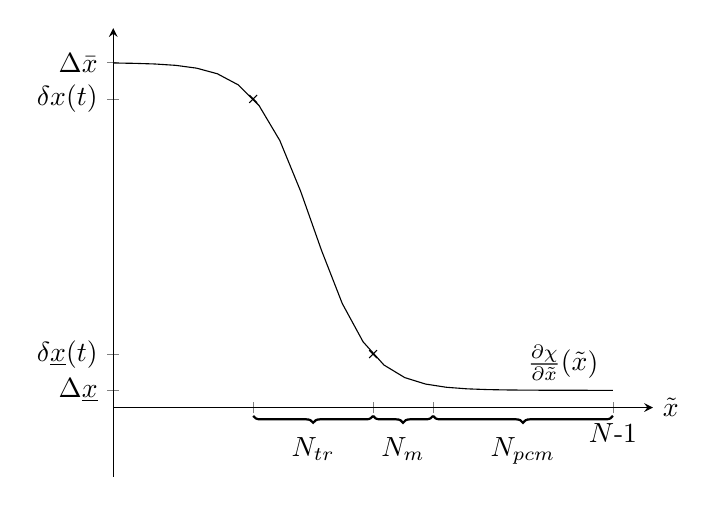
\begin{tikzpicture}
	\begin{axis}[
	axis x line = middle,
	axis y line = middle,
	xtick={7,13,16,25},
	ytick={0.05, 1., 0.155, 0.895},
	xticklabels={, , , $N\text{-}1$},
	yticklabels={$\Delta \underline{x}$, $\Delta \bar{x}$, $\delta \underline{x}(t)$, $\delta {x}(t)$},
	xmin=0, xmax=27,
	ymin=-0.2, ymax=1.1,
	xlabel=$\tilde{x}$, xlabel style={at=(current axis.right of origin), anchor=west},
	]
	\addplot [domain=0:25] {(1 - 0.05) / (exp(0.7*(x-10))+1) + 0.05} node[pos=0.9, above, sloped] {$\frac{\partial \chi}{\partial \tilde{x}}(\tilde{x})$};
	
	\draw [thick,decoration={brace,mirror,raise=3pt},decorate] 
	(axis cs:16,0) --
	node[below=7pt] {$N_{pcm}$} 
	(axis cs:25,0);
	
	\draw [thick,decoration={brace,mirror,raise=3pt},decorate] 
	(axis cs:13,0) --
	node[below=7pt] {$N_{m}$} 
	(axis cs:16,0);
	
	\draw [thick,decoration={brace,mirror,raise=3pt},decorate] 
	(axis cs:7,0) --
	node[below=7pt] {$N_{tr}$} 
	(axis cs:13,0);

	\addplot[only marks, mark=x, color=black] 
	table {7	0.895
	       13   0.155
	};	
	
	% L1
	\draw [loosely dashed] (0, 109.5) -- (70, 109.5);
	\draw [loosely dashed] (70, 20) -- (70, 109.5);	
	
	% L1 + L3
	\draw [loosely dashed] (0, 35.5) -- (130, 35.5);
	\draw [loosely dashed] (130, 20) -- (130, 35.5);	

	
	
	
	\end{axis}
	\end{tikzpicture}
	\caption{$\delta \underline{x}(t) := \Delta \underline{x} + (\Delta \bar{x} - \Delta \underline{x})\cdot(1-t)$, $\delta \bar{x}(t) := \Delta \underline{x} + (\Delta \bar{x} - \Delta \underline{x})\cdot t$}
	\label{fig:grid_size}
\end{figure}


\subsection{Analytical solution of reference side}

The measurement data for the residuum computation is given as a function dependent on the temperature at the reference crucible $T_{ref}^{\eta_i}$. Since we need to evaluate the solution of the heat equation (PCM side) at the corresponding time points $t_i$ it is necessary to calculate these.
This is done by applying Newton's method on the heat equation's solution of the reference side which can be solved analytically as follows. \\

As the crucible of the reference side is empty there is just the silver plate with a constant temperature coefficient $a$. The start and boundary conditions are equal to the ones of the PCM side. So the boundary value problem reads 

\begin{subequations}
	\begin{empheq}[box=\widefbox]{align}
		\frac{\partial T}{\partial t}(x,t) & - a \cdot \frac{\partial^2 T}{\partial x^2}(x,t) = 0 \label{eq:analytical_soln_pde} \\
		T(0,t) & = T_0 + \beta \cdot t \label{eq:analytical_soln_bc_neumann} \\
		\frac{\partial T}{\partial x}(L_1,t) & = 0 \label{eq:analytical_soln_bc_dirichlet}  \\
		T(x,0) & = T_0 
	\end{empheq}
\end{subequations}

The first step is a separate ansatz of the solution function $T(x,t)$ with $\bar{T}(x,t)$ satisfying the boundary conditions:

\begin{align}
	{T}(x,t) = \bar{T}(x,t) + \Gamma(x,t) \\
	\bar{T}(x,t) = A(t) + B(t) \cdot x
\end{align}

Inserting the boundary conditions and a coefficient comparison in $x$ gives

\begin{align}
	\bar{T}(0,t) = T_0 + \beta \cdot t = A(t) \\
	\frac{\partial \bar{T}}{\partial x}(L_1,t) = 0 \cdot x = B(t)
\end{align}

\begin{equation}
	\Rightarrow \bar{T}(x,t) = T_0 + \beta \cdot t
\end{equation}


By construction this leads to homogenous boundary conditions of $\Gamma(x,t)$:

\begin{align}
	T(0,t) & = \bar{T}(0,t) + \Gamma(0,t) = T_0 + \beta \cdot t + \Gamma(0,t) \stackrel{\eqref{eq:analytical_soln_bc_dirichlet}}{=} T_0 + \beta \cdot t \\
	 &\Rightarrow \Gamma(0,t) = 0 \\[2ex]
	\frac{\partial T}{\partial x}(L_1,t) & = \underbrace{\frac{\partial \bar{T}}{\partial x}(L_1,t)}_{= 0} + \frac{\partial \Gamma}{\partial x}(L_1,t) \stackrel{\eqref{eq:analytical_soln_bc_neumann}}{=} 0 \\
	 &\Rightarrow \frac{\partial \Gamma}{\partial x}(L_1,t) = 0
\end{align}


Inserting $\bar{T}$ and $\Gamma$ into \eqref{eq:analytical_soln_pde} gives

\begin{align}
	\frac{\partial \bar{T}}{\partial t} + \frac{\partial \Gamma}{\partial t} - a \left[ \frac{\partial^2 \bar{T}}{\partial x^2} + \frac{\partial^2 \Gamma}{\partial x^2} \right] = 0
\end{align}
	

	
	
With $\frac{\partial \bar{T}}{\partial t} = \beta$, $\frac{\partial^2 \bar{T}}{\partial x^2} = 0$ and

\begin{align}
T(x,0) & = \underbrace{\bar{T}(x,0)}_{T_0} + \Gamma(x,0) = T_0 \\
& \Rightarrow \Gamma(x,0) = 0
\end{align}

this leads to the boundary value problem in $\Gamma(x,t)$

\begin{subequations}
	\begin{empheq}[box=\widefbox]{align}
		\frac{\partial \Gamma}{\partial t}(x,t) - a \cdot \frac{\partial^2 \Gamma}{\partial x^2}(x,t) & = - \beta =: \bar{q} \label{eq:analytical_soln_pde_gamma} \\
		\Gamma(0,t) & = 0 \label{eq:analytical_soln_bc_neumann_gamma} \\
		\frac{\partial \Gamma}{\partial x}(L1,t) & = 0 \label{eq:analytical_soln_bc_dirichlet_gamma}  \\
		\Gamma(x,0) & = 0 =: \bar{f}
	\end{empheq}
	\label{eq:analytical_soln_gamma}
\end{subequations}


The homogeneous solution (i.e. $\bar{q}=0$) can be obtained by an ansatz of seperation of variables $\Gamma(x,t) = \mathcal{T}(t) \cdot X(x)$, \eqref{eq:analytical_soln_pde_gamma} is then equivalent to

\begin{equation}
	\dot{\mathcal{T}} X = a \mathcal{T} X'' \quad \Leftrightarrow \quad \frac{1}{a} \frac{\dot{\mathcal{T}}}{\mathcal{T}} = \frac{X''}{X} = const =: - \lambda
\end{equation}


since the LHS $\sfrac{\dot{\mathcal{T}}}{{\mathcal{T}}}$ just depends in $t$ and the RHS $\sfrac{X''}{X}$ just depends on $x$. 

The solution of the ordinary differential equation $X'' = - \lambda \cdot X$ is

\begin{equation}
	X(x) = c_1 \cdot \sin(\sqrt{\lambda} x) + c_2 \cdot \cos(\sqrt{\lambda} x)
\end{equation}

where $c_1$ and $c_2$ are determined by the boundary conditions $X(0) = 0$ and $X'(L_1) = 0$:

\begin{align}
	X(0) = c_2 \stackrel{!}{=} 0 \\
	X'(L_1) = \left. c_1 \sqrt{\lambda} cos(\sqrt{\lambda} x) \right|_{x=L_1} = c_1 \sqrt{\lambda} cos(\sqrt{\lambda} L_1) \stackrel{!}{=} 0 \\
	\Rightarrow \sqrt{\lambda_n} = \frac{(2n -1)\pi}{2 L_1} \qquad n=1,2,...
\end{align}

The general solution of $X_n(x)$ is then given by

\begin{equation}
	\tilde{X}_n(x) = c_1 \cdot \sin\left(\frac{(2n -1)\pi}{2 L_1} \cdot x\right) =: c_1 \cdot X_n(x)
\end{equation}

In order to solve the non-homogeneous boundary value problem \eqref{eq:analytical_soln_gamma} $\Gamma$, $\bar{q}$ and $\bar{f}$ are expanded in a Fourier series with $X_n(x)$ as basis where $c_1$ is incorporated in the corresponding Fourier coefficient:

\begin{subequations}
	\centering
	\begin{align}
		\Gamma(x,t) & = \sum_{n=1}^{\infty} \mathcal{T}_n(t) X_n(x) \\
		\bar{q}(x,t) & = \sum_{n=1}^{\infty} \bar{q}_n(t) X_n(x) \\
		\bar{f}(x) & = \sum_{n=1}^{\infty} \bar{f}_n X_n(x)
	\end{align}
\end{subequations}

The Fourier coefficients $\bar{q}_n(t)$ and $\bar{f}_n$ are then computed by

\begin{subequations}
	\begin{align}
		\bar{q}_n(t) & = \frac{\int_{0}^{L_1} \bar{q}(x,t) X_n(x) dx}{\int_{0}^{L_1} X_n^2(x) dx} \ \overbrace{=}^{\bar{q}=-\beta} \ - \frac{4 \beta}{\pi (2n - 1)} \\
		\bar{f}_n & = \frac{\int_{0}^{L_1} \bar{f}(x) X_n(x) dx}{\int_{0}^{L_1} X_n^2(x) dx} \ \underbrace{=}_{\bar{f}=0} 0
	\end{align}
\end{subequations}

Inserting this into \eqref{eq:analytical_soln_pde_gamma} gives us

\begin{align*}
	\sum_{n=1}^{\infty} \dot{\mathcal{T}}_n(t) X_n(x) - a \sum_{n=1}^{\infty} \mathcal{T}_n(t) X_n''(x) = \sum_{n=1}^{\infty} \bar{q}_n(t) X_n(x) \nonumber \\
	\stackrel{X'' = - \lambda X}{\Leftrightarrow} \ \ \sum_{n=1}^{\infty} \dot{\mathcal{T}}_n(t) X_n(x) + a \sum_{n=1}^{\infty} \lambda_n \mathcal{T}_n(t) X_n(x) = \sum_{n=1}^{\infty} \bar{q}_n(t) X_n(x)
\end{align*}

With a coefficient comparison in $X_n$ we get the inhomogeneous ODE

\begin{equation}
	\dot{\mathcal{T}_n}(t) + a \lambda_n \mathcal{T}_n(t) = \bar{q}_n(t)
	\label{eq:analytical_soln_inhomo_ode}
\end{equation}

where the solution of the homogeneous part (i.e. $\bar{q}_n(t) = 0$) is

\begin{equation}
	\mathcal{T}_n^h(t) = A_n \cdot e^{-a \lambda_n t}
\end{equation}

Applying the method of variation of constants by setting $A_n = A_n(t)$ and inserting in \eqref{eq:analytical_soln_inhomo_ode} gives

\begin{align}
	\dot{A_n}(t) & = \bar{q}_n(t) \cdot e^{a \lambda_n t} = -\frac{4 \beta}{\pi (2n - 1)} e^{a \lambda_n \tau} \\
	\Rightarrow A_n(t) & = \int_{0}^{t} -\frac{4 \beta}{\pi (2n - 1)} e^{a \lambda_n \tau} d \tau + A_{n,c} \\
	& = -\frac{4 \beta}{\pi (2n - 1)} \frac{1}{a \lambda_n} \left[ e^{a \lambda_n t} - 1 \right] + A_{n,c}
\end{align}

The solution of the inhomogeneous ODE \eqref{eq:analytical_soln_inhomo_ode} then is
\begin{align}
	\mathcal{T}_n(t) & = A_n(t) \cdot e^{-a \lambda_n t}  \\
	& = -\frac{4 \beta}{\pi (2n - 1)} \frac{1}{a \lambda_n} \left[1 - e^{-a \lambda_n t} \right] + A_{n,c} e^{- a \lambda_n t} \nonumber
\end{align}

The remaining unknown $A_{n,c}$ is determined by considering the Fourier series of the starting condition

\begin{equation}
	\Gamma(x,t) = \sum_{n=1}^{\infty} \mathcal{T}_n(0) X_n(x) = \sum_{n=1}^{\infty} \bar{f}_n X_n(x) = \bar{f}(x)
\end{equation}

From $\mathcal{T}_n(0) = A_{n,c}$, $\bar{f}_n=0$ and again a coefficient comparison it follows that

\begin{equation}
	A_{n,c} = 0
\end{equation}

Finally the solution of the boundary value problem \eqref{eq:analytical_soln_pde} of the reference side reads as

\begin{align}
	& \ \ T(x,t) = \bar{T}(x,t) + \Gamma(x,t) \nonumber \\
	\Leftrightarrow \ \ & T(x,t) = T_0 + \beta \cdot t + \sum_{n=1}^{\infty} \mathcal{T}_n(t) X_n(x) \nonumber \\[1ex]
	\Leftrightarrow \ \ & \raalign{}{T(x,t) = T_0 + \beta \cdot t - \sum_{n=1}^{\infty} \left\{ \frac{4 \beta}{\pi (2n - 1)} \frac{1}{a \cdot \lambda_n} \left[ 1 - e^{- a \lambda_n t} \right] \cdot \sin(\sqrt{\lambda_n} \cdot x) \right\}} \label{eq:analytical_soln_final_formula}
\end{align}


\todo{Fehleranalyse bzgl Konvergenz in $n$?}


\section{Parameter estimation of specific heat capacity $c_p$}





\subsection{Parametrization of $c_p$}
Since in the end we want to estimate the specific heat capacity $c_p$ we need a parametrization with enough degrees of freedom in order to generate appropriate functions. 

\subsubsection{NURBS}
In early stages of work we used Non-Uniform Rational B-Splines (NURBS). The generated curve $C(u) = \{C^x(u), C^y(u) \} \in \mathbb{R}^2$ is defined by

\begin{equation}
	C(u) = \frac{\sum_{i=0}^{n} N_{i,p}(u) \omega_i P_i }{\sum_{i=0}^{n} N_{i,p}(u) \omega_i} \qquad a \le u \le b
\end{equation}

where $P_i = \{ P_i^x, P_i^y \} \in \mathbb{R}^2$ are called control points, $\omega_i$ are weights for each control point and $N_{i,p}(u)$ are the B-Spline basis functions. These are defined recursively by

\begin{align}
	N_{i,p}(u) = & \frac{u - u_i}{u_{i+p} - u_i} N_{i,p-1}(u) + \frac{u_{i+p+1} - u}{u_{i+p+1} - u_{i+1}} N_{i+1,p-1}(u) \label{eq:NURBS_basis_polynomial} \\[1ex]
	N_{i,0} = &
	\begin{cases}
		1 \quad \text{if } u_i \le u < u_{i+1} \\
		0 \quad \text{otherwise}
	\end{cases} \nonumber
\end{align}

where $u_i$ are the elements of the knot vector

\begin{equation}
	U = \{u_0,...,u_m\}=\{a,...,a,u_{p+1},...,u_{m-p-1},b,...,b\}.
\end{equation}

With this formulation there are $n+1$ control points, $p$ is the order of the basis functions and the order of the resulting curve is defined by $p+1$. The interval $[a,b]$ is arbitrary in the sense that for $C(u=a)=P_0$,  $C(u=b)=P_n$ and $u \in (a,b)$ are points between depending on the knot vector.\\

In our experimental setup we used a NURBS order of $4$, i.e. $p=3$. $a=0$ and $b=1$ so $u \in [0,1]$ and the knot vector is linearly increasing, i.e. $U = \{ 0,0,0,0,\frac{1}{n p},\frac{2}{n p},...,\frac{n p - 1}{n p},1,1,1,1 \}$. All control points contribute equally such that $\omega_i=1 \ \forall \ i$. With these settings it holds that $C(u) \in \mathcal{C}^2$.

Since $C(u)$ is a parametrized curve we get a function $c_p(T)$ by using $C^x(u)$ as the domain of definition (temperature) and $C^y(u)$ as the co-domain ($c_p$). Evaluating $C(u)$ on an appropriate fine grid for values of $u$ and subsequently piecewise linear interpolation gives the wanted quantity $c_p(T)$.
The x-coordinates of the control points were fixed on a predefined grid with $P_i^x < P_{i+1}^x$ to guarantee a well-defined function.
As optimization variables we used the corresponding y-coordinates $P_i^y$.

\subsubsection{Fraser-Suzuki Peak}


\begin{align}
	c_p(T) =
	\begin{cases}
		h \cdot \exp \left\{ - \frac{\ln(r)}{\ln(sr)^2} \cdot \left[ \ln\left( 1 + (T-z) \cdot \frac{sr^2 - 1}{wr \cdot sr} \right) \right]^2 \right\} \ & \text{for } \ T < z - \frac{wr \cdot sr}{sr^2 - 1} \\
		0 \ & \ \text{else}
	\end{cases}
	\label{eq:fraser_suzuki}
\end{align}



\subsubsection{Linear combination of Gaussian functions}
As we switched for the derivative computation with respect to the optimization variables from finite differences to IND, implementation problems with NURBS occurred. 
The case structure of the basis polynomial \eqref{eq:NURBS_basis_polynomial} conducts to switch the RHS of the differential equation. This is only supported by the $condassign(a,b,c,d)$ function which assigns $a=c$ if $b>0$ and $a=d$ else. Additionally to $N_{i,0}$ the denominators need this $condassign$ command in order to check for a division by zero. 
Furthermore the piecewise interpolation of the resulting curve $C(u)$ could be realized as well with the $condassign$ command but in total this leads to a lot of unnecessary numerical operations and makes the program quite complex. \\
An alternative simple parametrization which is similar flexible than NURBS is a linear combination of Gaussian functions which is stated in \eqref{eq:parametrization_linear_comb_Gauss}. Per Gaussian there are three optimization variables: Amplitude $A_i$, a shift in the $T$-axis $T_{\text{offset}_i}$ and the standard deviation $\sigma_i$. Additionally there is a linear and constant part with variables $m$ and $b$. So in total there are $3 \cdot n_{\text{Gauss}} + 2$ optimization variables. \\


\begin{equation}
	c_p(T) = \sum_{i=1}^{n_{\text{Gauss}}} A_i \exp\left(- \frac{(T - T_{\text{offset}_i})^2}{\sigma_i^2}\right) + m \cdot T + b
	\label{eq:parametrization_linear_comb_Gauss}
\end{equation} \\

An example $c_p(T)$ function generated by this parametrization is shown in Fig. \ref{fig:parametrization_example_linear_comb_gauss}


\begin{figure}[H]
	\centering
	\includegraphics[width=0.8\textwidth]{/home/argo/masterarbeit/fits_data/old_Constantan/2017-10-05_00:14:13_407_0,3Kmin_L1=15_L3=0,35/c_p(T).png}
	\caption{blubb}
	\label{fig:parametrization_example_linear_comb_gauss}
\end{figure}









\subsection{Optimization problem}


\begin{align}
	\min_{p_{c_p}} \ & \sum_{i=1}^{n_{MP}} \left|\left|  \varPhi_{q}^{PCM,in}(T(t_i;T_0,p_{c_p})) - \varPhi_q^{\eta_i} \right|\right|_2^2 \\
	s.t. \ & \quad \  \dot{T} = f(T,t;p_{c_p}) \nonumber \\
	& T(0) = T_0 \nonumber
\end{align}


\begin{figure}[H]
	\centering
	\begin{tikzpicture}
	\begin{axis}[domain=0:65,
	samples=100,
	xmin=0, xmax=70,
	ymin=0.,	 
	axis lines=left,
	xtick={40},
	xticklabels={$t_i$},
	ytick={0.7, 3.7},
	yticklabels={$T_0$, $T_{ref}^{\eta_i}$},
	xlabel=$time$, xlabel style={at=(current axis.right of origin), anchor=west},
	ylabel=\empty
	]
	
	\addplot+[color=black, mark=none] {0.7 + 0.1*x}
	node[pos=0.87, above, sloped] {$T_{{furnace}}$};
	
	\addplot+[color=black, mark=none] {0.7 + 0.1*x - (1 - exp(-0.11*x)}
	node[pos=0.95, below, sloped] {$T_{{ref}}^{{sim}}$};
	
	\addplot[only marks, mark=x, color=black] 
	table {40 3.7
	};	
	
	\draw [loosely dashed] (0, 370) -- (400, 370);
	\draw [loosely dashed] (400, 0) -- (400, 370);	
	
	\end{axis}
	\end{tikzpicture}
	\caption{}
	\label{fig:}
\end{figure}


\section{Numerical experiments and results}
\subsection{Parameter estimation using finite differences and NURBS parametrization}



\subsection{Error analysis of spatial discretization grid}
\todo{Zugang zu Rechencluster und Referenz mit aequidistantem grid berechnen}


\subsection{Parameter estimation using Fraser-Suzuki parametrization}

\subsection{Parameter estimation using linear combination of Gaussians parametrization}



\section{Discussion}



\begin{thebibliography}{9}

\bibitem{diss_jan}
	 Adjoint-based algorithms and numerical methods for sensitivity generation and optimization of large scale dynamic systems, 
	 Jan Albersmeyer, 2010,
	 http://www.ub.uni-heidelberg.de/archiv/11651
\bibitem{DSC_buch}
	Differential Scanning Calorimetry of Polymers: physics, chemistry, analysis, technology,
	Vladimir A. Bershtein, Victor M. Egorov,
	1994
\bibitem{diss_DSC}
	Kalorimetrische Methoden zur Bestimmung
	der Enthalpie von Latentwärmespeichermaterialien
	während des Phasenübergangs,
	Stefan Hiebler, Dissertation an der technischen Universität München, 2006
	
\bibitem{numerik1_skript_koerkel}
	Numerische Mathematik 1 Vorlesungsskript, 
	Prof. Dr. Stefan Körkel, 2015

\bibitem{ADOL-C}
	ADOL-C: 1
	A Package for the Automatic Differentiation
	of Algorithms Written in C/C++,
	Version 2.1.12-stable, November 2010,
	Andrea Walther and Andreas Griewank
	
\bibitem{pcm_solar_cells}
	Improving the performance of solar panels by the use of phase-change materials,
	Pascal Biwole, Pierre Eclache, Frederic Kuznik,
	World Renewable Energy Congress 2011 - Sweden
	
\bibitem{lit:waerme_und_stoffuebertragung}
	Wärme- und Stoffübertragung,
	Hans Dieter Baehr, Karl Stephan,
	9. Auflage, 2016
	
\bibitem{DIN_11357}
	DIN EN ISO 11357, 
	Kunststoffe –
	Dynamische Differenz-Thermoanalyse (DSC)
  
\end{thebibliography}

\end{document}